\documentclass[9pt,academicons]{article}

\usepackage{CADA}
\usepackage{calrsfs}
\usepackage{color}
\usepackage[table]{xcolor}
\definecolor{light-gray}{gray}{0.8}
\definecolor{light-light-gray}{gray}{0.9}

\title{Notes on the CAD-Compatible Conversion of Multi-Sided Surfaces}

\begin{document}


\maketitle

\authorSection{
	\anAuthor{P\'eter Salvi}{0000-0003-2456-2051}{1},
	\anAuthor{Tam\'as V\'arady}{0000-0001-9547-6498}{2} and
	\anAuthor{Alyn Rockwood}{}{3}
}

\affiliationSection{
	\anAffiliation{1}{Budapest University of Technology and Economics}{salvi@iit.bme.hu}
	\anAffiliation{2}{Budapest University of Technology and Economics}{varady@iit.bme.hu}
	\anAffiliation{3}{Boulder Graphics LLC, USA}{alynrock@gmail.com}
}

\correspondingAuthor{P\'eter Salvi}{salvi@iit.bme.hu}

\abstract{
We investigate genuine multi-sided surface representations that can be
converted into standard tensor product format, such as NURBS.  Multi-sided
patches offer versatility in shape design, and permit smooth, watertight connections
between adjacent patches using prescribed cross-derivatives; however, they can seldom be
utilized by the majority of CAD/CAM systems, which handle surfaces
only in standard data formats.
Tensor product surfaces, on the other hand, may be too rigid for shape design,
and trimmed patches can only be smoothly connected up to user-defined tolerances.
% Tensor product surfaces are more rigid for shape design,
% and smoothly connecting trimmed surface patches is tolerance driven and
% generally requires extra effort.
This motivates the search for schemes that benefit from both representations.

We analyze four multi-sided surface representations that allow precise
conversion into tensor product format, namely S-patches, Warren's patch,
Kato's patch and a variant of the Charrot--Gregory patch. We compare these schemes
from various aspects; in particular, we deal with surface equations, singularities,
degrees of the converted surfaces, the control structure built and the computational
efficiency of the conversion. Several examples help to gain deeper insights into
the problem.
}

\keywords{multi-sided surfaces, trimmed surfaces, S-patch, Charrot--Gregory patch} 

\doi{10.14733/cadaps.2021.156-169}

\section{INTRODUCTION}
\label{sec:intro}
The majority of aesthetic objects are represented by free-form shapes, and modeling these
naturally involves multi-sided (i.e., non-four-sided) surfaces.  The
mathematical representation of such patches is still an active area in CAGD, and although
a great variety of approaches have been published, none of the genuine $n$-sided
formulations have been standardized so far.

On the other hand, commercial CAD/CAM systems and related application programs only accept
data in standard formats, such as tensor product NURBS surfaces. For this reason, a
widely applied practice is to convert multi-sided surfaces into a CAD-compatible
representation either by (i)~approximating them with larger quadrilaterals and
\emph{trimming} away the exterior part beyond the boundaries, or (ii)~\emph{splitting}
them into smaller four-sided patches.
Both techniques have their deficiencies. They only approximate the original multi-sided
surface, and in general, trimming cannot ensure even precise $C^0$ continuity between
adjacent patches. In the splitting scheme the subdividing curves in the interior
reduce the overall continuity of the surface.

Ideally, we would like to have an $n$-sided patch that:
\begin{enumerate}[label=\roman*),leftmargin=3\parindent]
\item can be used for design (has intuitive controls),
\item can be attached to adjacent patches with $G^1$ or higher continuity,
\item and can also be represented \emph{accurately} as a tensor product NURBS surface.
\end{enumerate}

The above problem can be resolved, if the multi-sided surfaces can be represented as rational
polynomials of two parametric variables. Then they can be directly converted into
NURBS form, without either changing the surfaces or harming continuity. The result will be
a collection of \emph{watertight trimmed surfaces}.
 
Some of the well-known multi-sided schemes allow computing a trimmed rational bi-parametric
representation. Our goal in this paper is to review these and discuss the difficulties of
the conversion process. We are going to provide further insights into specific
computational and geometric problems that have not been discussed elsewhere and are
useful for analyzing the ``pros and cons'' of these representations.

The paper is structured as follows. In Section~\ref{sec:multisided},
we review four pure multi-sided schemes, and investigate their conversions to tensor product NURBS.
In Section~\ref{sec:discussion}, issues of the conversion process are discussed in details,
with emphasis on the quality of the generated control network, and its relation to singularities.
Some more complex test examples and comparisons follow in Section~\ref{sec:tests},
showing actual high-degree examples with control grids,
and a summary of our findings concludes the paper.

\section{MULTI-SIDED SURFACES}
\label{sec:multisided}
In the following, we are going to review four multi-sided representations:
the S-patch~\cite{Loop:1989}, and the surface schemes of Warren~\cite{Warren:1992},
Kato~\cite{Kato:1991}, and Charrot \& Gregory~\cite{Charrot:1984}.
Our conversion approach is presented in
Sections~\ref{subsubsec:parameters}--\ref{subsubsec:conversion}
specifically for S-patches, but it will be adapted to other representations in
Sections~\ref{subsec:kato} and~\ref{subsec:charrot}.

\subsection{S-Patch}
\label{subsec:spatch}
The S-patch of Loop \& DeRose~\cite{Loop:1989} is a generalization of the B\'ezier triangle, or,
more precisely, a B\'ezier simplex mapping from $(n-1)$D to 3D, where the $n$ coordinates of the
domain are supplied by generalized barycentric coordinates. The \emph{depth} ($d$) of an S-patch
is the number of \emph{de Casteljau} steps required to evaluate a surface point, i.e.,
something similar
to the degree of a B\'ezier triangle (but not the degree of the S-patch itself).
S-patches have many nice properties, and are known to be convertable into tensor product
rational B\'ezier surfaces of degree $d(n-2)$.

An $n$-sided S-patch is defined over a regular $n$-gon, parameterized by generalized
barycentric coordinates $\mathbf{\lambda}=(\lambda_1,\dots,\lambda_n)$~\cite{Floater:2015}.
Its control
points $\{P_\mathbf{s}\}$ are labeled by $n$ non-negative integers $\mathbf{s}=(s_1,\dots,s_n)$,
whose sum is the depth of the surface. Then points on the surface are defined by
the equation
\begin{equation}
  \label{eq:spatch}
  S(\mathbf{\lambda})=\sum_{\mathbf{s}}P_\mathbf{s}\cdot B_\mathbf{s}^d(\mathbf{\lambda})
  =\sum_{\mathbf{s}}P_\mathbf{s}\cdot {d\choose\mathbf{s}}\cdot\prod_{i=1}^n\lambda_i^{s_i},
\end{equation}
where $B_\mathbf{s}^d(\mathbf{\lambda})$ are Bernstein polynomials with multinomial coefficients,
and the sum is computed over all possible values of $\mathbf{s}$.

One drawback of this representation is its large number of control points, which renders it
inconvenient for interactive design. For example, a five-sided patch of depth 5 has 126 control
points, while a 4-sided quintic tensor product patch has only 36. A possible workaround is to use a
$G^1$ \emph{frame} (Fig.~\ref{fig:spatch-ribbon})
for design that defines the tangent planes at the boundaries.
After increasing the depth by 3, these boundary constraints can be interpolated~\cite{Loop:1990},
and the remaining interior control points can be set by some heuristic to generate a smooth
surface~\cite{Salvi:2019:KEPAF}, see
Figures~\ref{fig:spatch-cnet-ribbon}--\ref{fig:spatch-cnet-full}.
\begin{figure}
  {
    \begin{subfigure}{0.32\textwidth}
      \centering
      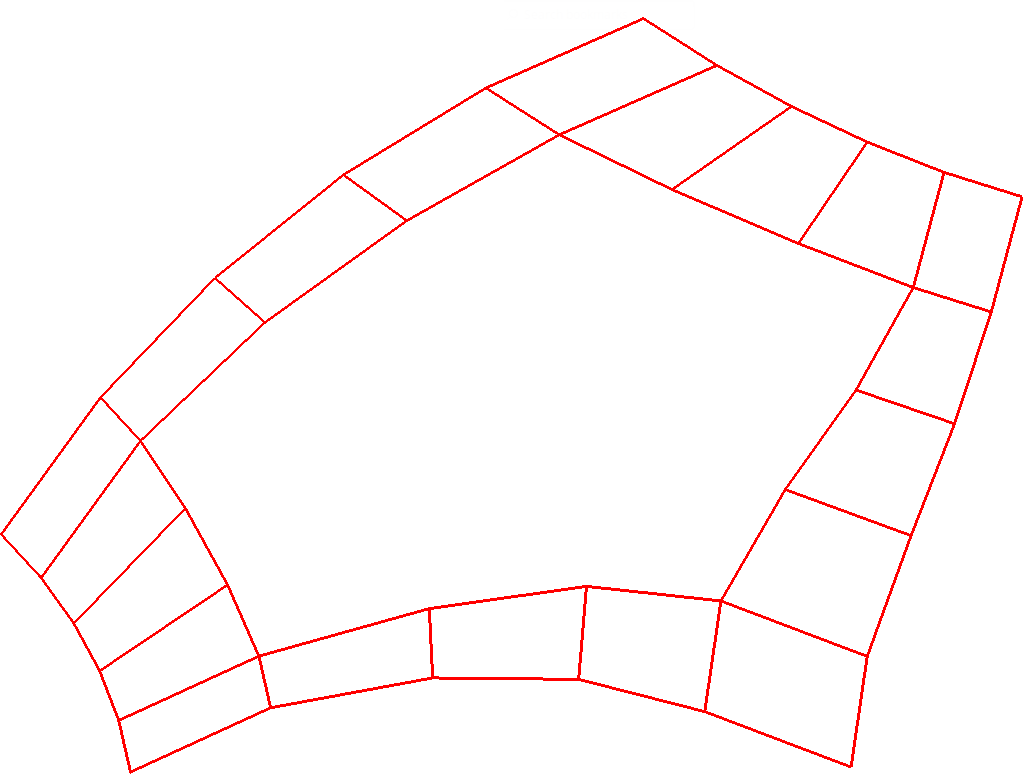
\includegraphics[width = 0.95\textwidth]{images/5-5-bezier-ribbon.png}
      \caption{$G^1$ frame}
      \label{fig:spatch-ribbon}
    \end{subfigure}
    \hfill
    \begin{subfigure}{0.32\textwidth}
      \centering
      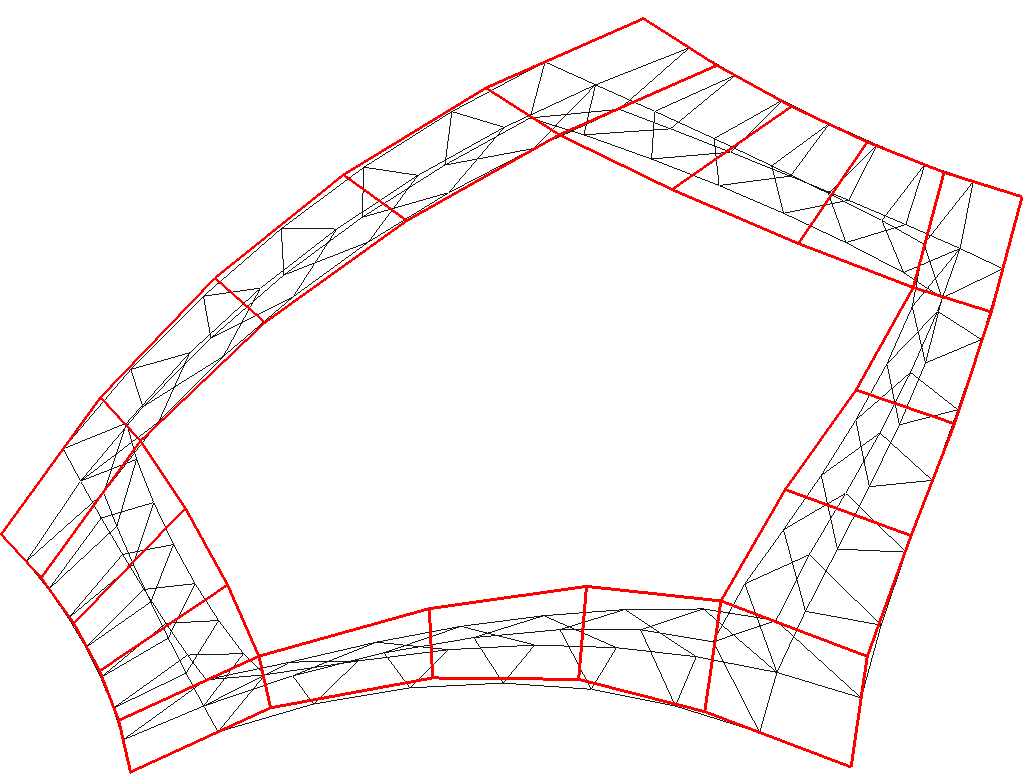
\includegraphics[width = 0.95\textwidth]{images/5-5-cnet-ribbon.png}
      \caption{Control points by $G^1$ constraints}
      \label{fig:spatch-cnet-ribbon}
    \end{subfigure}
    \hfill
    \begin{subfigure}{0.32\textwidth}
      \centering
      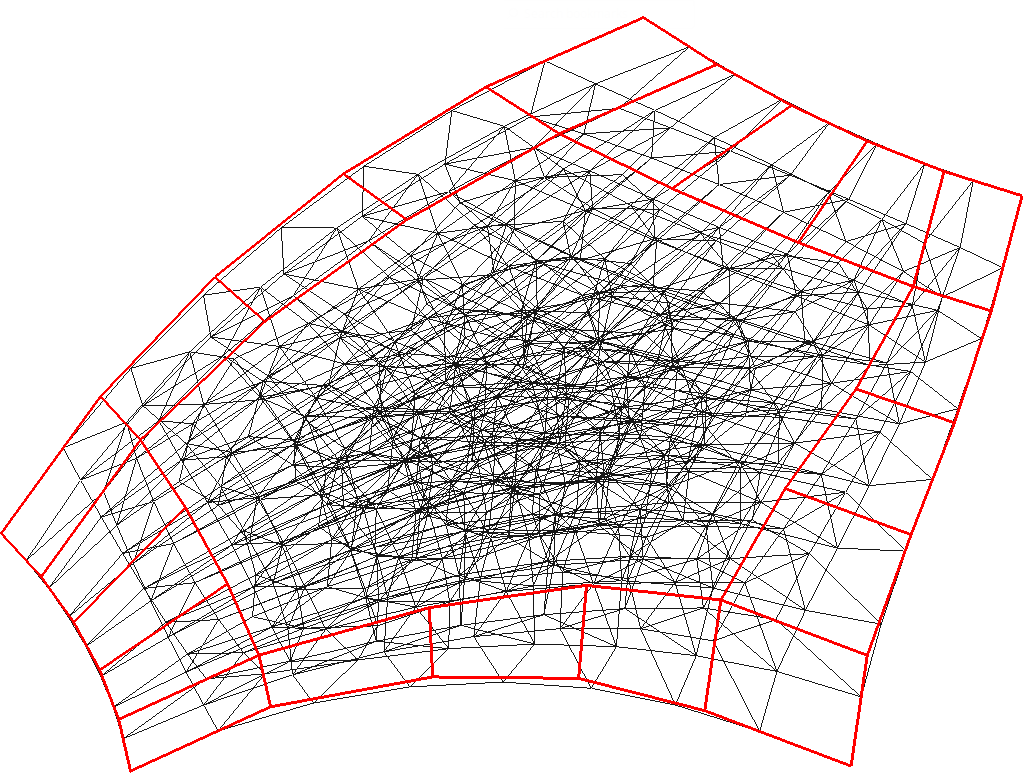
\includegraphics[width = 0.95\textwidth]{images/5-5-cnet-full.png}
      \caption{All control points}
      \label{fig:spatch-cnet-full}
    \end{subfigure}
  }
  \caption{Creating an S-patch from a $G^1$ frame.}
  \label{fig:spatch}
\end{figure}

The CAD-compatible conversion presented in~\cite{Loop:1989} is a two-step process:
first convert the surface into a
four-sided S-patch, and then to a tensor product patch. The first step is based on the
composition of B\'ezier simplexes~\cite{DeRose:1988}, which has very high complexity.
Even using a more efficient simplex composition
algorithm~\cite{DeRose:1993}, converting a modest-sized S-patch
still requires minutes of computation on today's machines~\cite{Salvi:2019:WAIT}.

\subsubsection{Parameterization Using Implicit Line Equations}
\label{subsubsec:parameters}
Here we propose an alternative conversion process. Since a B\'ezier simplex is polynomial,
the only problem is how to express the generalized barycentric coordinates as a rational polynomial
of the $(u,v)$ parameters on the 2D domain. Using Wachspress coordinates~\cite{Floater:2015},
$\{\lambda_i\}$ can be expressed as
\begin{equation}
  \label{eq:wachspress}
  \lambda_i(u,v) = \prod_{\substack{j=1\\j\notin\{i-1,i\}}}^nh_j(u,v) \quad\bigg/\quad
                   \sum_{k=1}^n\prod_{\substack{j=1\\j\notin\{k-1,k\}}}^nh_j(u,v),
\end{equation}
where the indexing is cyclic, and $h_j(u,v)$ is a \emph{distance function}
from the $j$-th side of the domain polygon. For the sake of brevity,
we will use the notation
\begin{equation}
  \label{eq:prod-h}
  H_J^k(u,v)=\prod_{\substack{j=1\\j\notin{J}}}^nh_j^k(u,v),
\end{equation}
where $J$ is an index set to exclude certain terms.
Then $\lambda_i(u,v)=H_{i-1,i}^1(u,v)/\sum_{k=1}^nH_{k-1,k}^1(u,v)$.

The distance function should vanish at the base domain edge, and increase monotonically
as we get farther from it.
The implicit
equation of the line containing the base edge is suitable for this purpose,
and is also a linear polynomial,
so the Wachspress coordinates can be expressed as rational polynomials of degree $n-2$. We
normalize the distances so they take on the value 1 at the vertices adjacent to the side.

Formally, let
\begin{equation}
  V_i=\left(\frac{1}{2}+\frac{1}{2}\cos(2\pi\cdot i/n),
            \frac{1}{2}+\frac{1}{2}\sin(2\pi\cdot i/n)\right),\quad i=1\dots n
\end{equation}
denote the vertices of the regular $n$-sided domain inside the $[0,1]\times[0,1]$ square,
see Figure~\ref{fig:domain}. % Yes, not the same orientation, get over it!
Since a line $L$ is defined by the implicit equation $L(u,v)=Au+Bv+C=0$, the coefficients can
be unambiguously defined by three equations. We define $n$ lines
$L_i$ ($i=1\dots n$) by the following constraints:
\begin{align}
  L_i(V_{i-1})&=L_i(V_i)=0, & L_i(V_{i-2})&=L_i(V_{i+1})=1.
\end{align}
(Note that because of the symmetry of the regular polygon, the above four equations constrain
only three degrees of freedom.) The distance function is then defined as
\begin{equation}
  h_i(u,v)=L_i(u,v),
\end{equation}
see constant parameter lines in Figure~\ref{fig:h}.
\begin{figure}
  \begin{subfigure}{0.30\textwidth}
    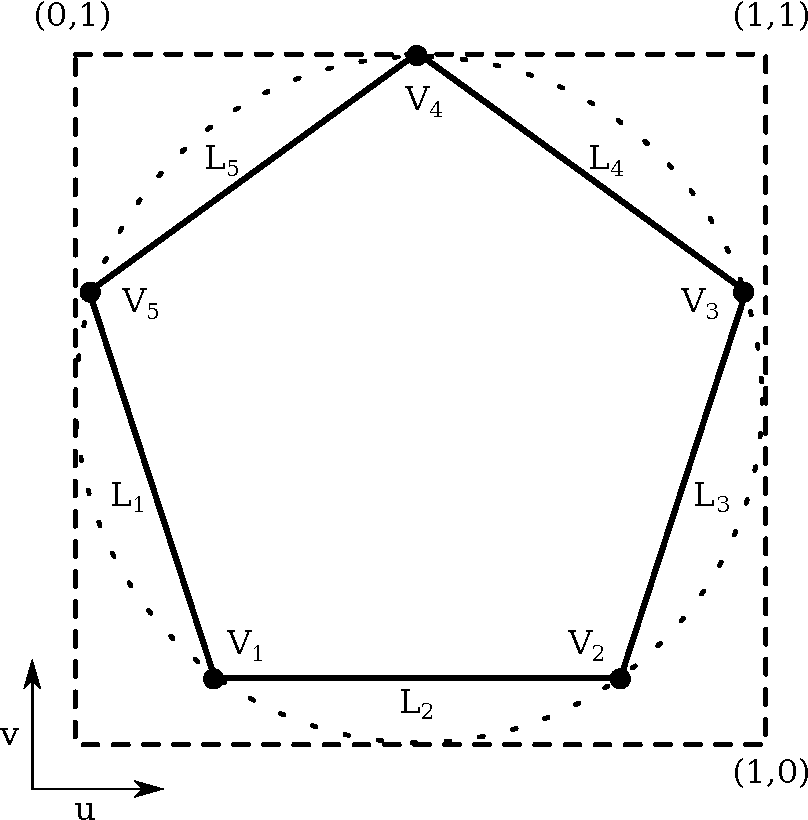
\includegraphics[width = \textwidth]{images/domain.pdf}
    \caption{Domain}
    \label{fig:domain}
  \end{subfigure}
  \hfill
  \begin{subfigure}{0.30\textwidth}
    \begin{minipage}[b][5cm][b]{\textwidth}
      \centering
      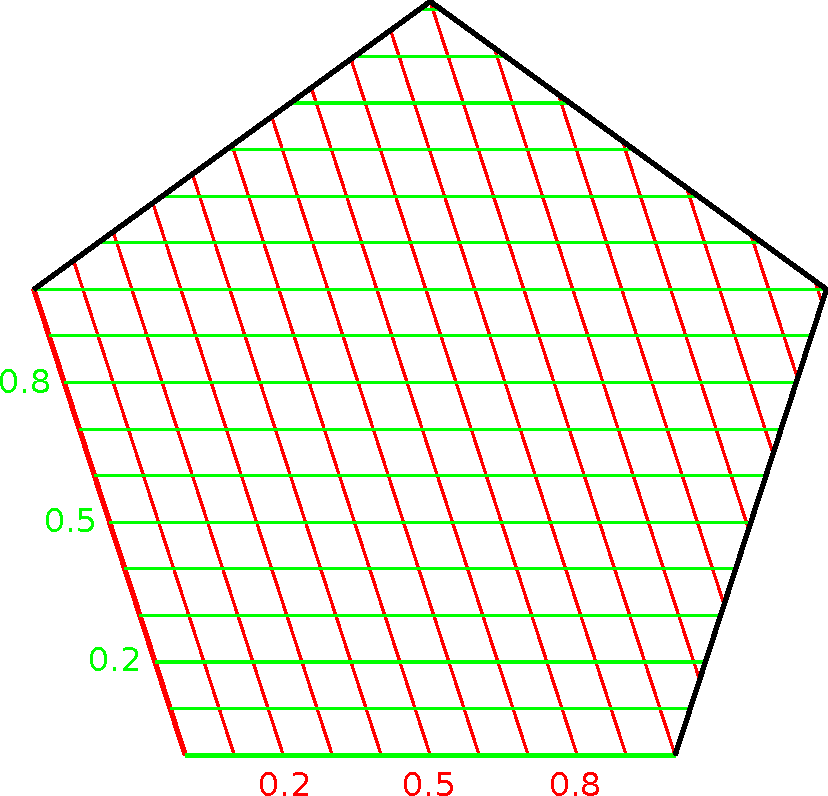
\includegraphics[width = \textwidth]{images/h-params.pdf}
      \vspace*{-2mm}
    \end{minipage}
    \caption{$h_i$ isolines for two sides}
    \label{fig:h}
  \end{subfigure}
  \hfill
  \begin{subfigure}{0.3\textwidth}
    \begin{minipage}[b][5cm][b]{\textwidth}
      \centering
      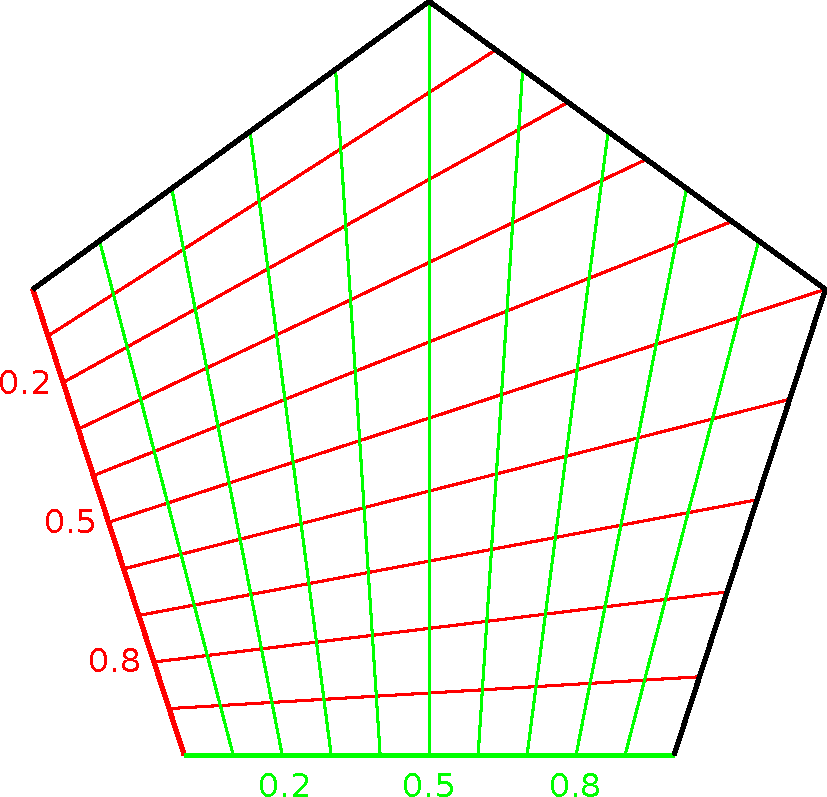
\includegraphics[width = \textwidth]{images/s-params.pdf}
      \vspace*{-2mm}
    \end{minipage}
    \caption{$s_i$ isolines for two sides}
    \label{fig:s}
  \end{subfigure}
  \caption{Parameterization.}
  \label{fig:parameters}
\end{figure}

\subsubsection{Conversion to NURBS}
\label{subsubsec:conversion}
With the above definition of generalized barycentric coordinates,
the patch equation~(\ref{eq:spatch}) becomes a rational vector polynomial in $u$ and $v$.
Since $|\mathbf{s}|=\sum_{i=1}^ns_i=d$, all terms of the sum have the same denominator,
\begin{equation}
  \left(\sum_{k=1}^nH_{k-1,k}^1(u,v)\right)^d,
\end{equation}
which is a polynomial of degree $d(n-2)$. It is easy to see that the rational degree $\delta$ of
the whole patch is also the same.

This means that we can represent an $n$-sided S-patch of depth $d$ by a rational B\'ezier
surface of $\delta\times\delta$ degrees. In order to determine the positions of the control points,
we still need to change from the power basis to the Bernstein basis.

Assuming that the coefficients of a bi-degree $\delta$ polynomial $p(u,v)$
are given in a matrix $M$ such that
\begin{equation}
  \label{eq:power}
  p(u,v)=
  \left[\begin{array}{ccccc}1&u&u^2&\dots&u^\delta\end{array}\right]
  M
  \left[\begin{array}{ccccc}1&v&v^2&\dots&v^\delta\end{array}\right]^\top,
\end{equation}
the B\'ezier coefficients are computed as $N=C^\top MC$, where $C=\{c_{ij}\}$ is
the upper triangular matrix with elements
\begin{equation}
  \begin{aligned}
    c_{ij}&={j\choose i}\bigg/{\delta\choose i}, & i,j&=0\dots\delta, & i&\leq j.
  \end{aligned}
\end{equation}
Then the same polynomial is expressed as
\begin{equation}
  \label{eq:bernstein}
  p(u,v)=
  \left[\begin{array}{cccc}B_0^\delta(u)&B_1^\delta(u)&\dots&B_\delta^\delta(u)\end{array}\right]
  N
  \left[\begin{array}{cccc}B_0^\delta(v)&B_1^\delta(v)&\dots&B_\delta^\delta(v)\end{array}\right]^\top.
\end{equation}
Control point positions and the corresponding weights are computed as homogeneous coordinates,
by calculating the coefficients for the numerator and denominator of Eq.~(\ref{eq:spatch})
separately, and assigning the latter as the extra \emph{weight} coordinate.

With this method, the B\'ezier control points of the tensor product representation
can be located by straightforward computation, which takes only milliseconds.

\subsection{Warren's Patch}
\label{subsec:warren}
Warren~\cite{Warren:1992} created multi-sided patches from B\'ezier triangles by assigning $0/0$
\emph{base points} to some of the control points, essentially cutting off corners, and thus
creating 5- and 6-sided surfaces; see an example in Figure~\ref{fig:warren-cnet}.
We can characterize Warren's patch with the number $m_i$ of control rows
``trimmed'' from each corner. Using the indices $\mathbf{s}=(s_1,s_2,s_3)$
introduced in Section~\ref{subsec:spatch},
\begin{equation}
  \begin{aligned}
    P_\mathbf{s}&=0/0, & \mathrm{when}\ &
    s_2+s_3<m_1\ \mathrm{or}\ s_3+s_1<m_2\ \mathrm{or}\ s_1+s_2<m_3.
  \end{aligned}
\end{equation}
For example, in Figure~\ref{fig:warren-cnet} two control rows are cut from two corners,
so $m_1=2$, $m_2=2$ and $m_3=0$.

\begin{figure}
  \begin{subfigure}{0.49\textwidth}
    \centering
    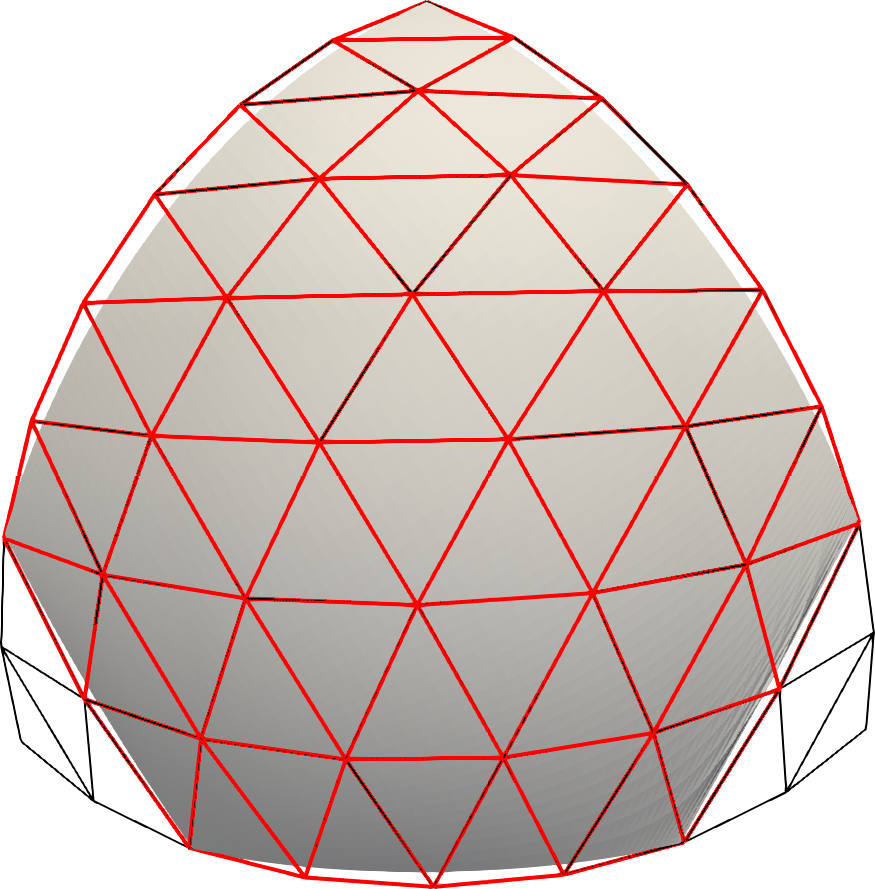
\includegraphics[width = 0.5\textwidth]{images/warren-cnet.png}
    \caption{Control points}
    \label{fig:warren-cnet}
  \end{subfigure}
  \hfill
  \begin{subfigure}{0.49\textwidth}
    \centering
    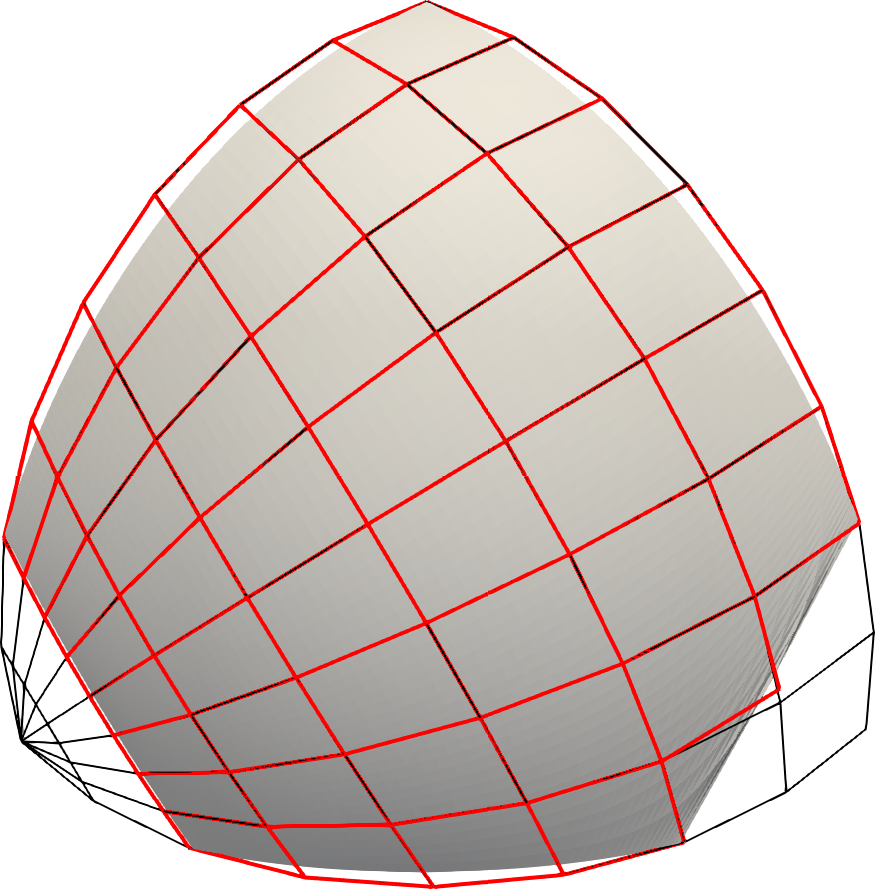
\includegraphics[width = 0.5\textwidth]{images/warren-quad.png}
    \caption{Conversion to NURBS}
    \label{fig:warren-quad}
  \end{subfigure}
  \caption{Warren's 5-sided patch.}
  \label{fig:warren}
\end{figure}
A simple NURBS conversion is also shown in the paper,
using the degenerate transformation
\begin{align}
  \lambda_1&=(1-u)v, & \lambda_2&=uv, & \lambda_3&=1-v.
\end{align}
Applying this to Eq.~(\ref{eq:spatch}) results in a tensor product surface; its control points
can be computed using Eqs.~(\ref{eq:power}--\ref{eq:bernstein}).
Figure~\ref{fig:warren-quad} shows an example. Note that the control points outside the
patch boundaries are actually base points and are drawn here only for better comprehension
of the control net structure.

A nice property of this patch is that the ``remaining'' control points define the behavior of the
boundary in the same way as in a normal B\'ezier triangle, i.e., the first control row defines
its position as a B\'ezier curve, the second its first derivatives etc.

It is important to see that not all degree configurations are available.
The example in Figure~\ref{fig:warren}, for example, has boundary curves with the
following degrees, starting from the bottom side: $[4,2,6,6,2]$. In the common case
when all boundaries have the same degree, a 6-sided patch is easily created from 
a triangle of degree $3d$, but due to its asymmetric construction,
a 5-sided patch always has edge curves of different degrees.
A $3d$-degree triangle suffices here, as well, but some of the boundaries need to be
degree elevated. For example, a 5-sided quintic patch can be generated from a 15-degree
B\'ezier triangle by cutting 5 control rows from two corners, resulting in boundaries of
degrees $[5,5,10,10,5]$, so two boundary curves need to be elevated to degree 10.

In addition, using control points with zero
weight is not a standard practice, and is not supported by many systems. Meshing
also presents a problem, as a uniform grid on the domain would result in distorted triangles,
since the ``trimmed'' boundaries correspond to corners of the domain triangle.

\subsection{Kato's Patch}
\label{subsec:kato}
Kato~\cite{Kato:1991} proposed a surface defined as the transfinite interpolation of boundary
curves with cross-derivatives:
\begin{equation}
  S_\mathrm{Kato}(u,v)=\sum_{i=1}^nR_i(s_i(u,v),h_i(u,v))\Gamma_i^{e}(u,v),
\end{equation}
where $\Gamma_i^{e}(u,v)$ is a singular blending function (see below), and
$R_i(s_i,h_i)$ is a quadrilateral \emph{ribbon} smoothly interpolating the $i$-th side.
The cross-degree of the ribbon
(and thus the number of cross-derivative constraints) is denoted by $e$.

Aside from the distance parameter $h_i$, defined as in Section~\ref{subsubsec:parameters},
this representation also uses a \emph{side parameter} $s_i$
that takes on values from 0 to 1 as it sweeps from one adjacent side to the other,
see Figure~\ref{fig:s}.
One such function is
\begin{equation}
  s_i(u,v)=\frac{L_{i-1}(u,v)}{L_{i-1}(u,v)+L_{i+1}(u,v)},
\end{equation}
which gives a rational polynomial parameterization.

The blending function is given as
\begin{equation}
  \Gamma_i^{e}(u,v)=H_i^{e+1}(u,v)\big/\sum_{k=1}^nH_k^{e+1}(u,v),
\end{equation}
with $H_i^{e+1}(u,v)$ defined as in Eq.~(\ref{eq:prod-h}).
Note that the denominator vanishes for the corner points of the domain polygon,
but the surface is well-defined there.

When the ribbons are given as B\'ezier surfaces of the form
\begin{equation}
  \label{eq:ribbon}
  R_i(s_i,h_i)=\sum_{j=0}^d\sum_{k=0}^{e}P_{j,k}^iB_j^d(s_i)B_k^{e}(h_i),
\end{equation}
with $P_{j,k}^i$ denoting the control points,
the whole patch becomes a rational polynomial, and can be converted to
a tensor product B\'ezier patch with rational degree $nd+(n-1)(e+1)+e$,
see Appendix~\ref{app:conversion-eqs} for the details.
In particular, using a $G^1$ frame ($e=1$), the degree will be $nd+2n-1$.

\subsection{Charrot--Gregory Patch}
\label{subsec:charrot}
The Charrot--Gregory patch~\cite{Charrot:1984} combines corner interpolants, but it can
also be formulated equivalently using ribbon surfaces~\cite{Salvi:2014}.
Let $I_{i-1,i}(s_{i-1},s_i)$ denote the corner interpolant based on sides $i-1$ and $i$,
parameterized by the corresponding side parameters.
(Note that on a regular domain the $s_i$ parameters defined above
will be the same as the radial parameterization in the original paper.)

The corner interpolant can be written as
\begin{equation}
  I_{i-1,i}(s_{i-1},s_i)=R_{i-1}(s_{i-1},s_i)+R_i(s_i,1-s_{i-1})-Q_{i-1,i}(s_{i-1},s_i),
\end{equation}
where $R_{i-1}$ and $R_i$ are linear ribbons (Eq.~(\ref{eq:ribbon}) with $e=1$),
and $Q_{i-1,i}$ is a correction patch defined by
\begin{equation}
  Q_{i-1,i}(s_{i-1},s_i)=P_{00}^i+s_id(P_{10}^i-P_{00}^i)+(1-s_{i-1})d(P_{01}^i-P_{00}^i)
  +s_i(1-s_{i-1})d^2(P_{11}^i-P_{10}^i-P_{01}^i+P_{00}^i).
\end{equation}

Finally, the Charrot--Gregory surface itself is formulated as
\begin{equation}
  S_\mathrm{CG}(u,v)=\sum_{i=1}^n I_{i-1,i}(s_{i-1}(u,v),s_i(u,v))\Gamma_{i-1,i}(u,v),
\end{equation}
where $\Gamma_{i-1,i}(u,v)$ is the blending function
\begin{equation}
  \Gamma_{i-1,i}(u,v)=H_{i-1,i}^2(u,v)\big/\sum_{k=1}^nH_{k-1,k}^2(u,v).
\end{equation}

Conversion is done the same way as in Section~\ref{subsubsec:conversion};
the converted patch is of degree $nd+2(n-2)$,
see details in Appendix~\ref{app:conversion-eqs}.
Note that the degree is relatively high because of the rational parameterization.
For triangular surfaces, we can use distance parameters instead,
thereby reducing the overall degree to $d+3$, see Appendix~\ref{app:triangular}.
Figure~\ref{fig:trebol} shows an example with one 6-sided and three 3-sided surfaces.
\begin{figure}
  \begin{subfigure}{.24\textwidth}
    \centering
    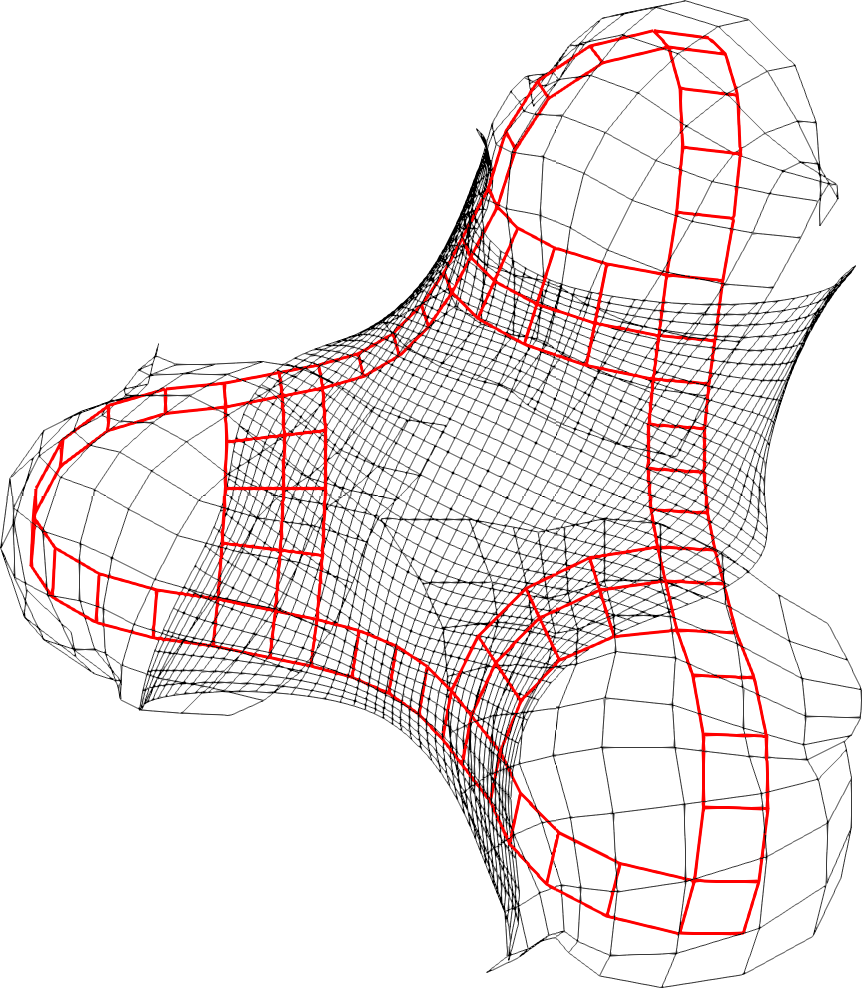
\includegraphics[height=.2\textheight]{images/trebol3-cnet.png}
    \caption{Control points}
    \label{fig:trebol-cnet}
  \end{subfigure}
  \hfill
  \begin{subfigure}{.24\textwidth}
    \centering
    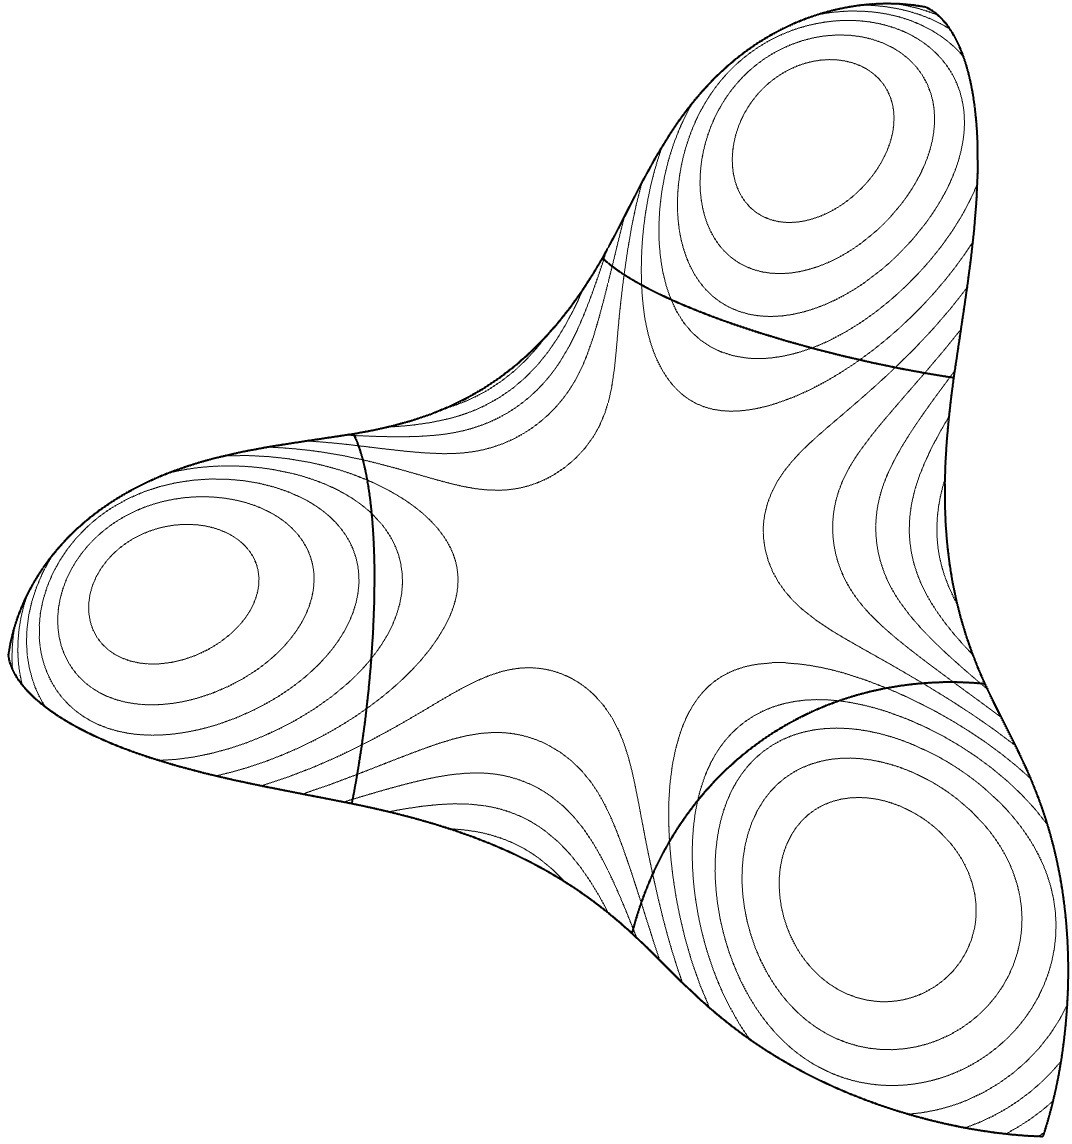
\includegraphics[height=.193\textheight]{images/trebol3-contour.jpg}
    \caption{Contours}
    \label{fig:trebol-contours}
  \end{subfigure}
  \hfill
  \begin{subfigure}{.24\textwidth}
    \centering
    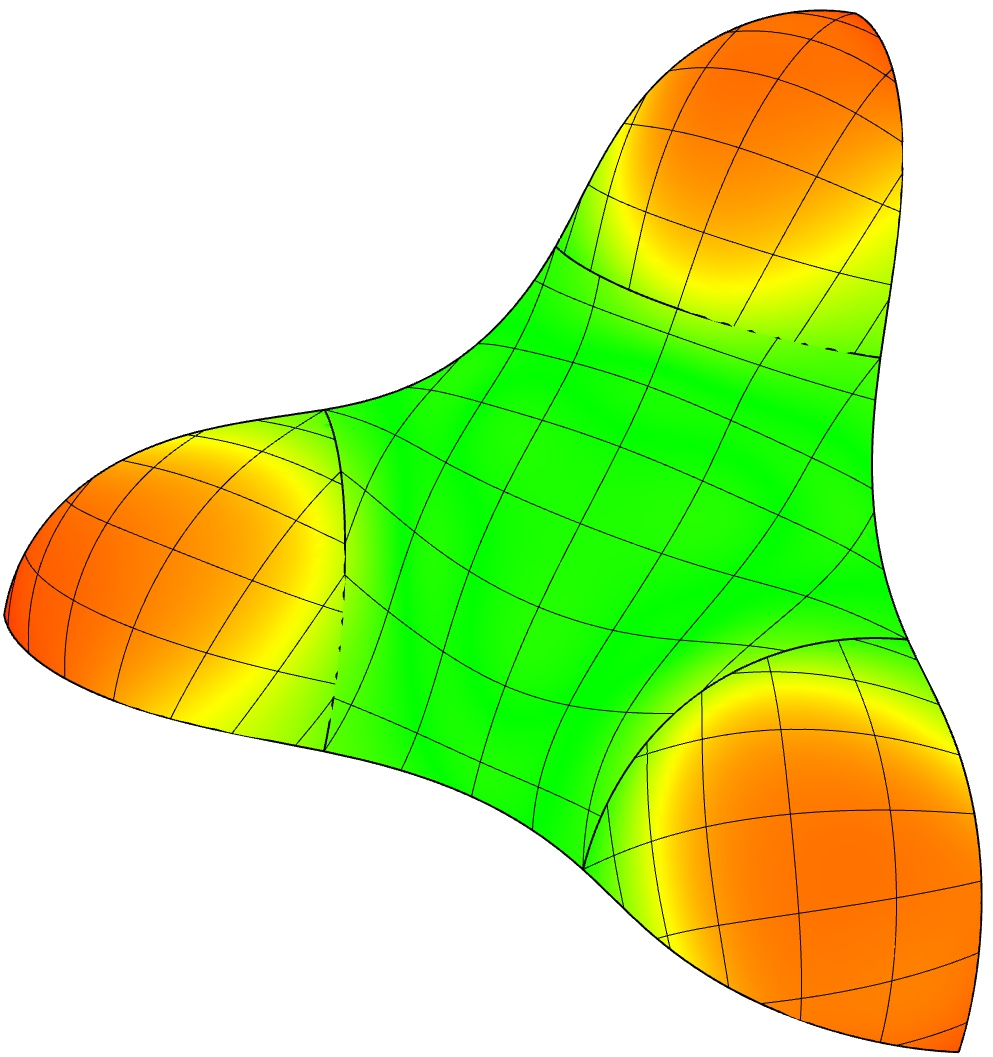
\includegraphics[height=.2\textheight]{images/trebol3-mean-iso.jpg}
    \caption{Mean curvature}
    \label{fig:trebol-mean}
  \end{subfigure}
  \hfill
  \begin{subfigure}{.24\textwidth}
    \centering
    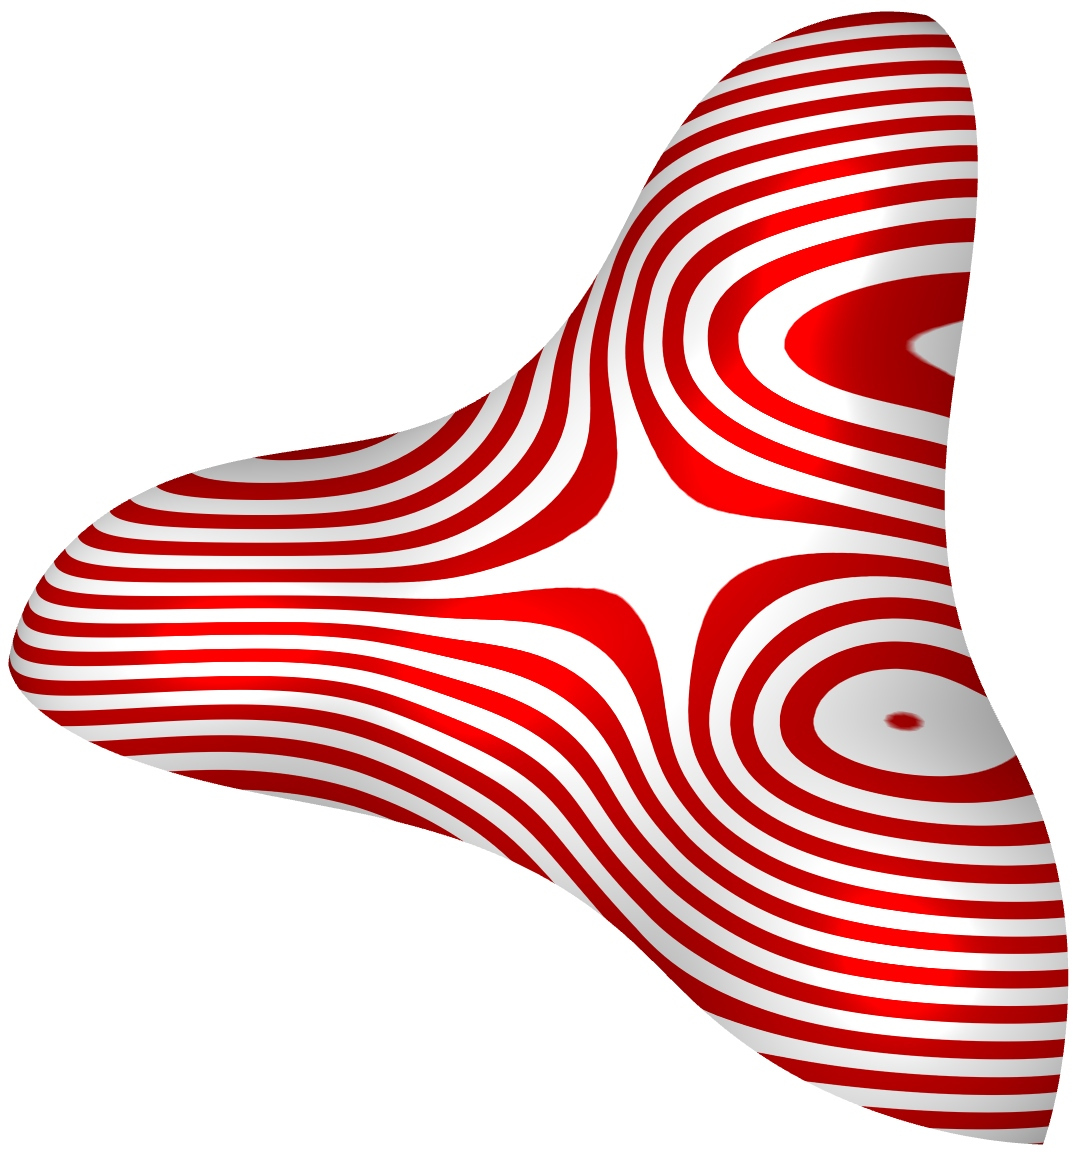
\includegraphics[height=.2\textheight]{images/trebol3-zebra.jpg}
    \caption{Zebra map}
    \label{fig:trebol-zebra}
  \end{subfigure}
  \caption{Trebol model.}
  \label{fig:trebol}
\end{figure}

\section{DISCUSSION}
\label{sec:discussion}
One aspect of the tensor product conversion we have not touched on before is the \emph{quality}
of the control net. Aside from Warren's patch, which has singular control points,
all the other representations have singularities in or outside their domains.
When a singular point is close to the domain of the tensor product patch (i.e., the unit square),
the control points in the vicinity show erratic behavior.

S-patches are singular on the circle that goes
through the intersections of the lines containing the domain edges,
as the denominator of Wachspress coordinates becomes zero on the
\emph{adjoint curve} of the domain, see details in~\cite{Floater:2015}.
The Charrot--Gregory patch is singular at lines parallel to the edges,
touching the adjoint circle at the intersection points, since
the denominator of $s_i$ vanishes.
Kato's patch also has these singularities, while it is also singular at the corners of the domain,
where the denominator of the blending function vanishes.

Figure~\ref{fig:singularities} illustrates this for 5-sided and 8-sided domains.
Here the blue rectangle represents the domain of the tensor product surface;
the dashed circle shows the singularities of S-patches,
while the red lines are the singularities of Charrot--Gregory and Kato patches.
The effect of these singularities depend on their proximity to the unit square
-- consequently quite disastrous for the 8-sided case,
see Figure~\ref{fig:8sided-default}.
\begin{figure}
  \begin{subfigure}{.45\textwidth}
    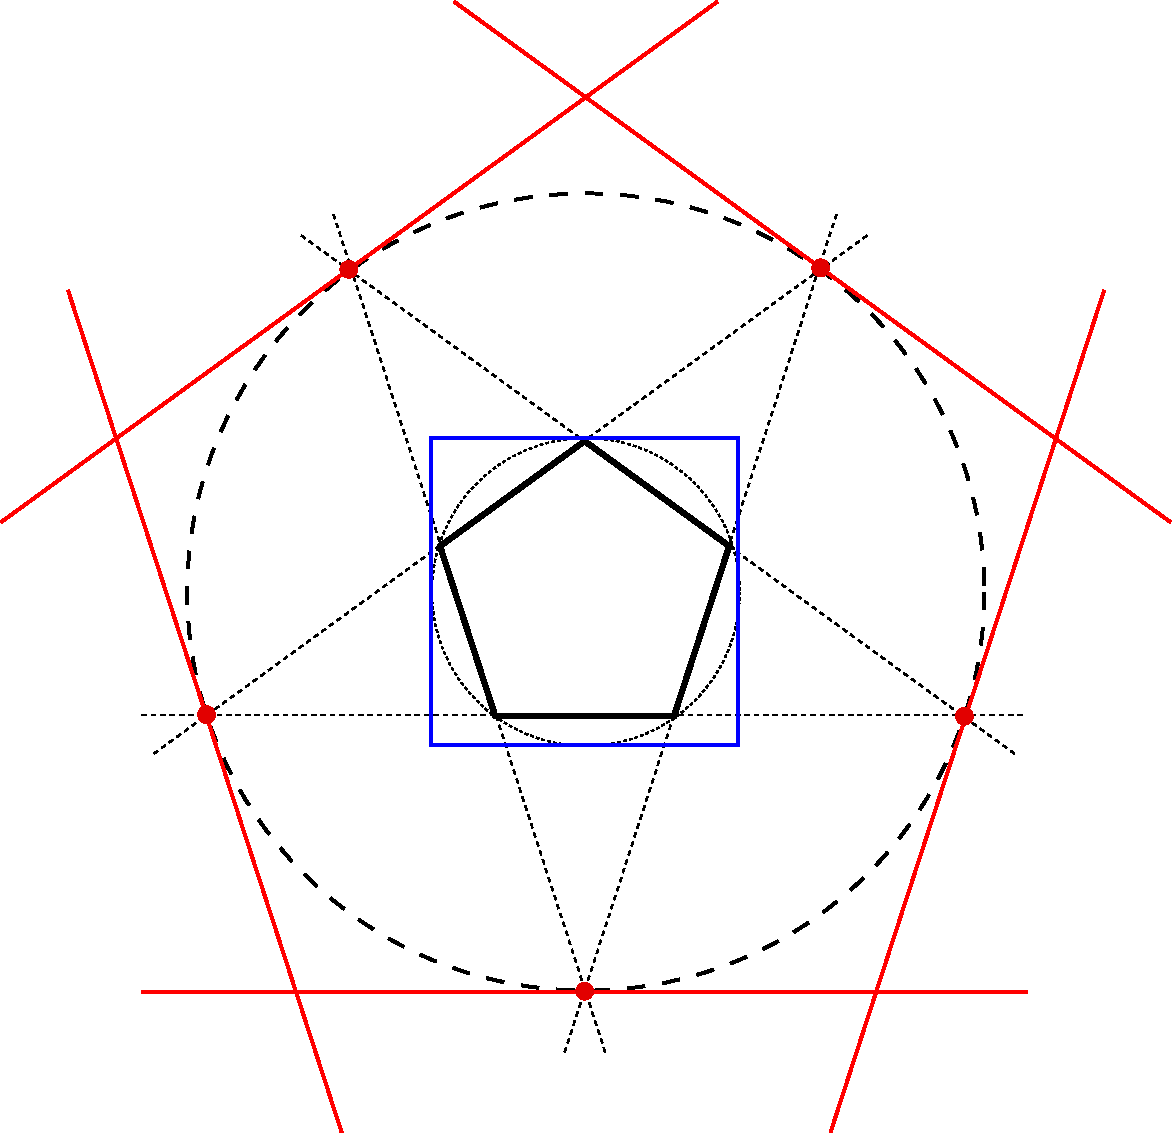
\includegraphics[width=\textwidth]{images/singularities.pdf}
    \caption{5-sided domain}
    \label{fig:singularities5}
  \end{subfigure}
  \hfill
  \begin{subfigure}{.45\textwidth}
    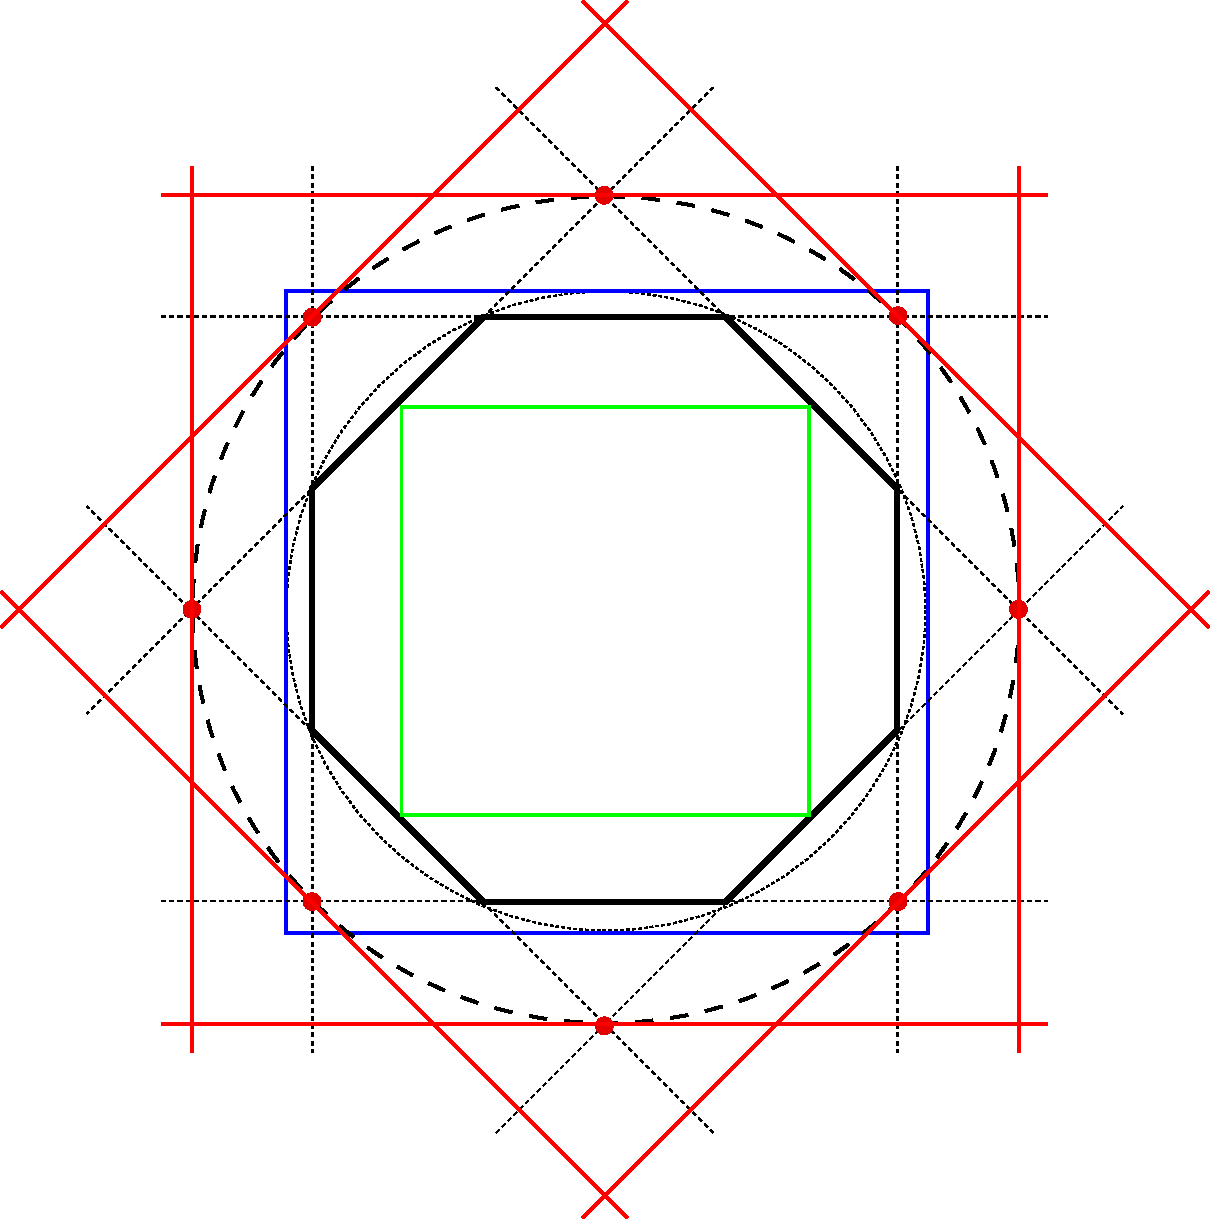
\includegraphics[width=\textwidth]{images/singularities2.pdf}
    \caption{8-sided domain}
    \label{fig:singularities8}
  \end{subfigure}
  \caption{Singularities around the domain.}
  \label{fig:singularities}
\end{figure}

We can summarize the effect of singularities on the different surface representations
as follows.
The triangular S-patch, which is not rational, has a
stable control structure, while for $n=5$ and $n=6$ some control points may
lie far from the multi-sided surface. For $n\geq 7$ the converted tensor product
surfaces are likely to have badly oscillating control points (possibly tending to infinity),
which may lead to numerical issues. The situation is better for the
Charrot--Gregory patch, where reliable control nets can be generated for $n\leq 6$.
The control grid of Kato's patch, and the above surfaces with more than 6 sides,
can hardly be used when converted to NURBS form.

We present a solution to this problem. Normally the multi-sided domain is inside the unit
square, so that the trimming curves will be inside the
surface, but if we lift this constraint, we can create a larger multi-sided domain,
thereby separating the unit square from the singularities. This means that the actual ``trimmed''
region will be outside the standard $[0,1]\times[0,1]$ domain; this may not be supported by some
applications, but the control structure will be close to the surface.
An example with an 8-sided patch is presented in Figure~\ref{fig:8sided-enlarged};
the green rectangle in Figure~\ref{fig:singularities8} shows
the unit square relative to the enlarged domain.
\begin{figure}
  \begin{subfigure}{.3\textwidth}
    \centering
    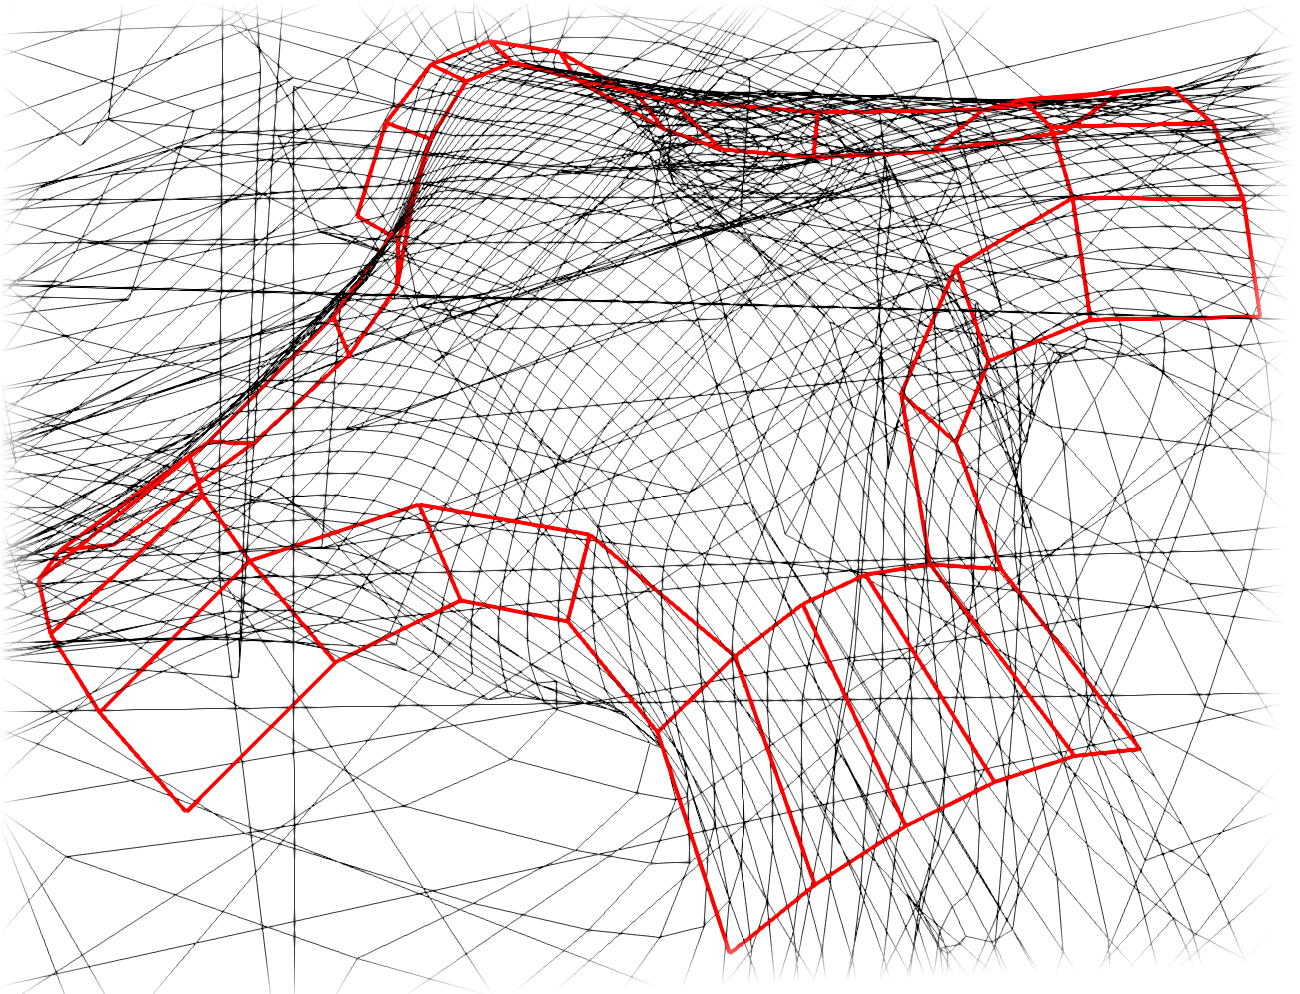
\includegraphics[width=\textwidth]{images/8sided-1.png}
    \caption{Control net (default domain)}
    \label{fig:8sided-default}
  \end{subfigure}
  \hfill
  \begin{subfigure}{.3\textwidth}
    \centering
    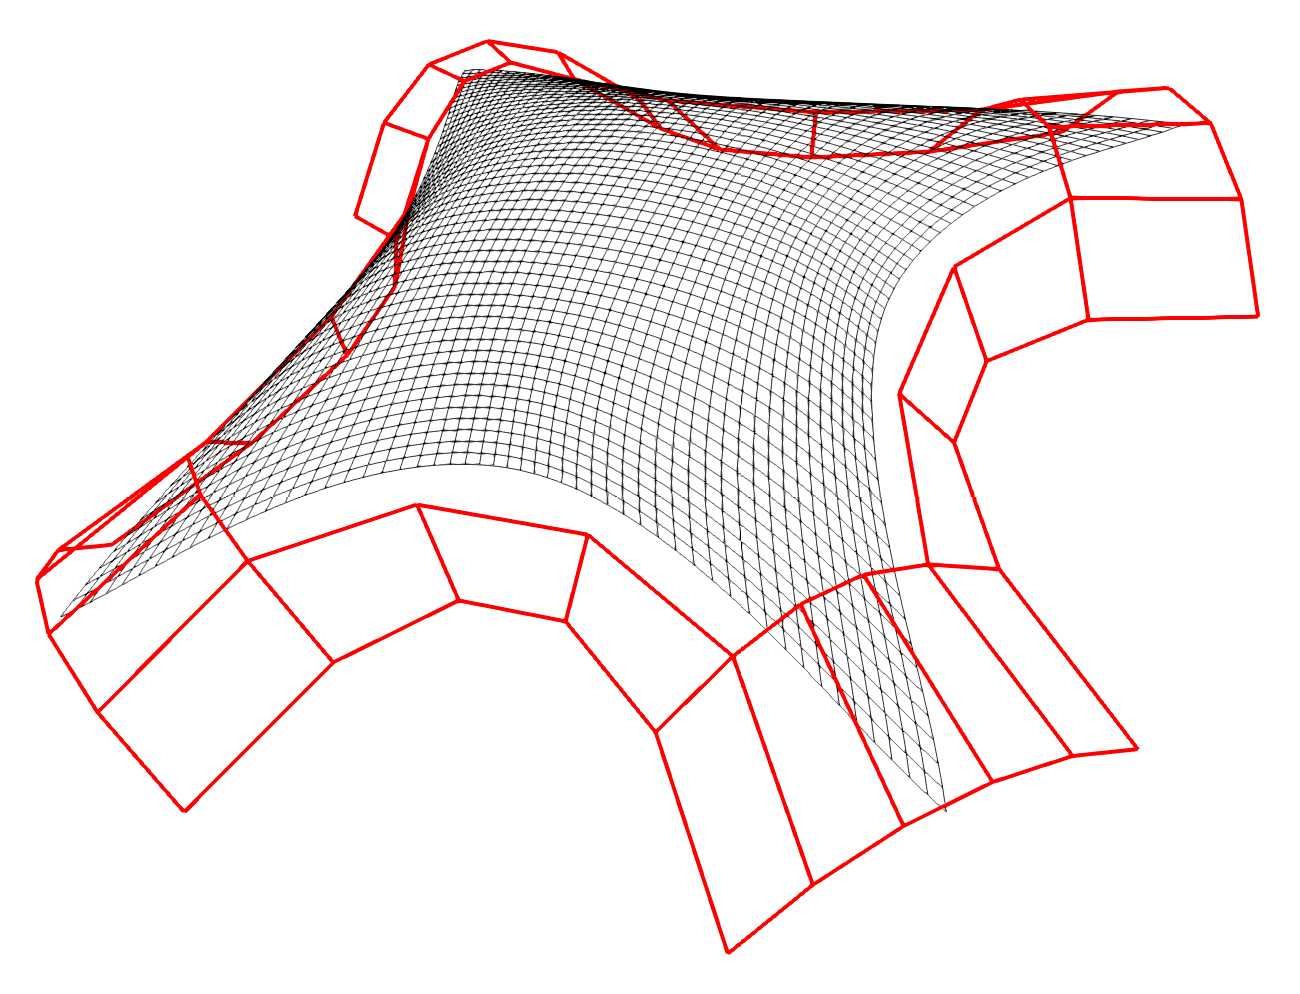
\includegraphics[width=\textwidth]{images/8sided-2.png}
    \caption{Control net (enlarged domain)}
    \label{fig:8sided-enlarged}
  \end{subfigure}
  \hfill
  \begin{subfigure}{.3\textwidth}
    \centering
    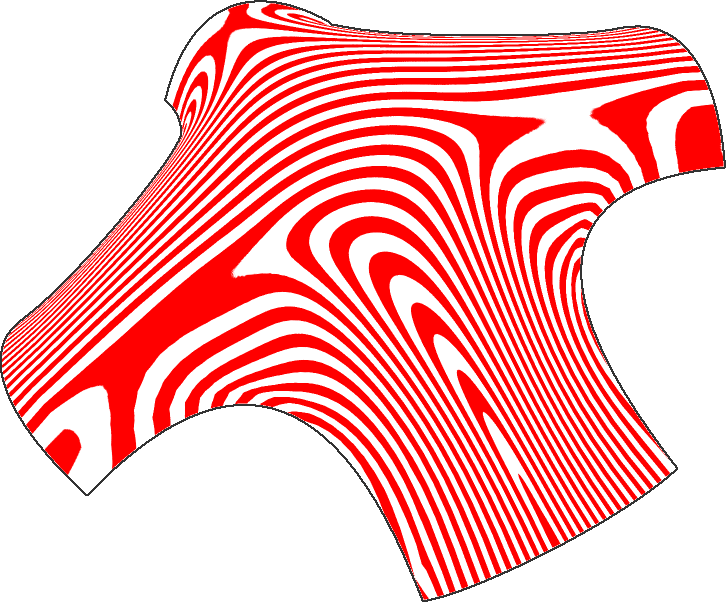
\includegraphics[width=.883\textwidth]{images/8sided-3.png}
    \caption{Isophote lines}
    \label{fig:8sided-iso}
  \end{subfigure}
  \caption{An 8-sided Charrot--Gregory patch.}
  \label{fig:8sided}
\end{figure}

\begin{figure}[!ht]
  {
    \hfill
    \begin{subfigure}{.26\textwidth}
      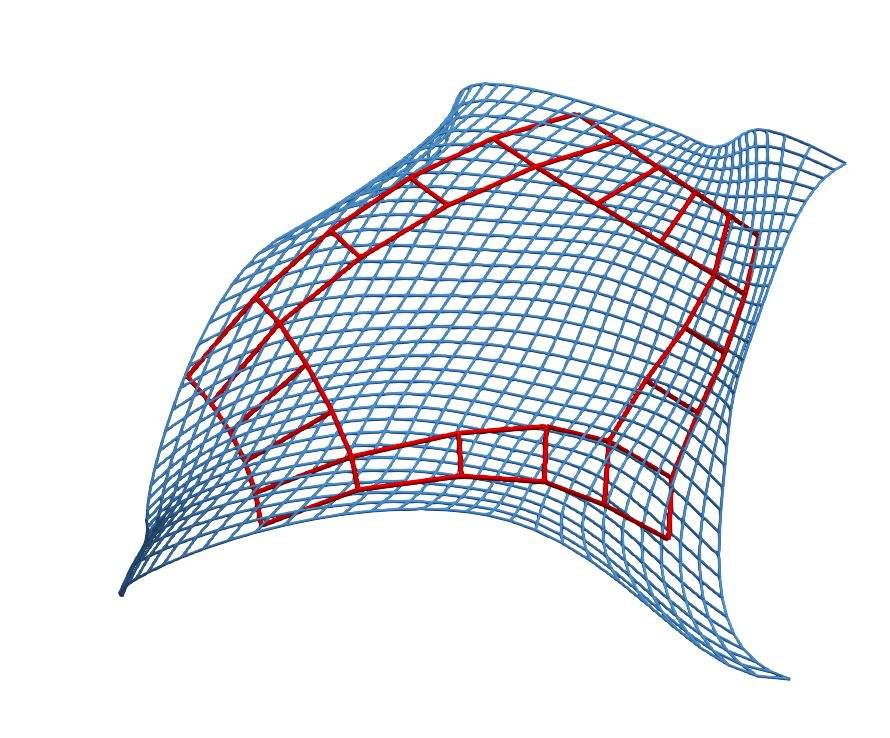
\includegraphics[width=\textwidth]{images/rotations/00.png}
      \caption{$\phi=0^\circ$}
    \end{subfigure}
    \hfill
    \begin{subfigure}{.26\textwidth}
      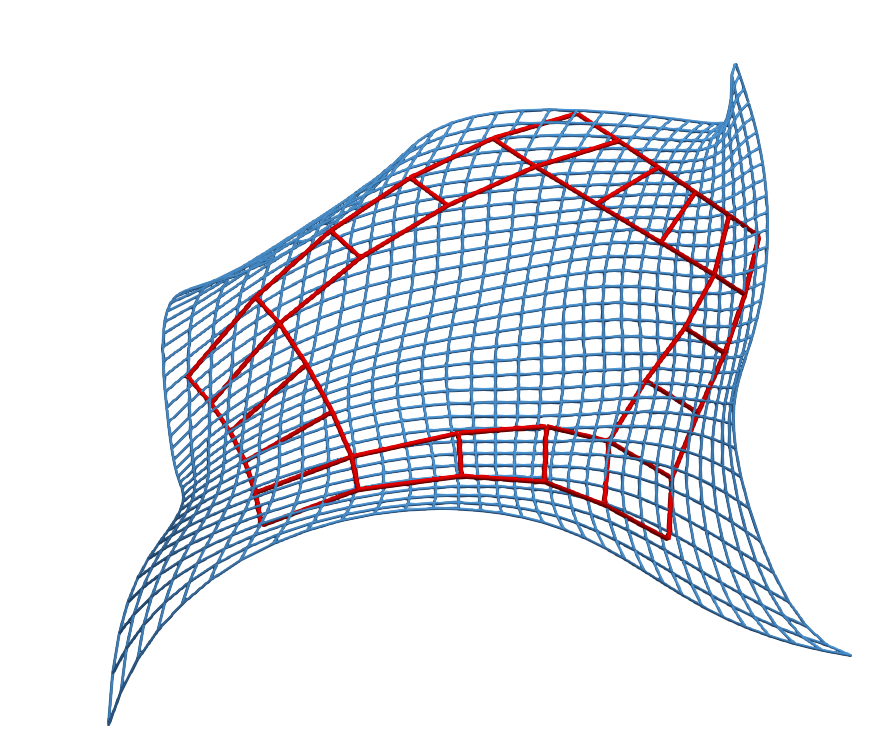
\includegraphics[width=\textwidth]{images/rotations/20.png}
      \caption{$\phi=20^\circ$}
    \end{subfigure}
    \hfill
    \begin{subfigure}{.26\textwidth}
      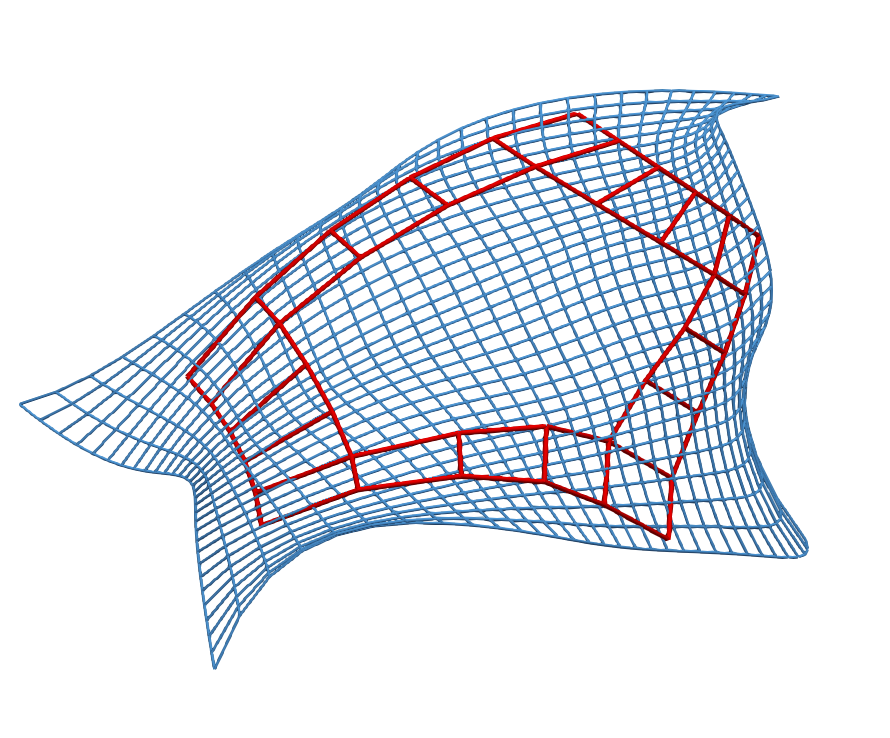
\includegraphics[width=\textwidth]{images/rotations/40.png}
      \caption{$\phi=40^\circ$}
    \end{subfigure}
    \hfill
  }

  {
    \hfill
    \begin{subfigure}{.26\textwidth}
      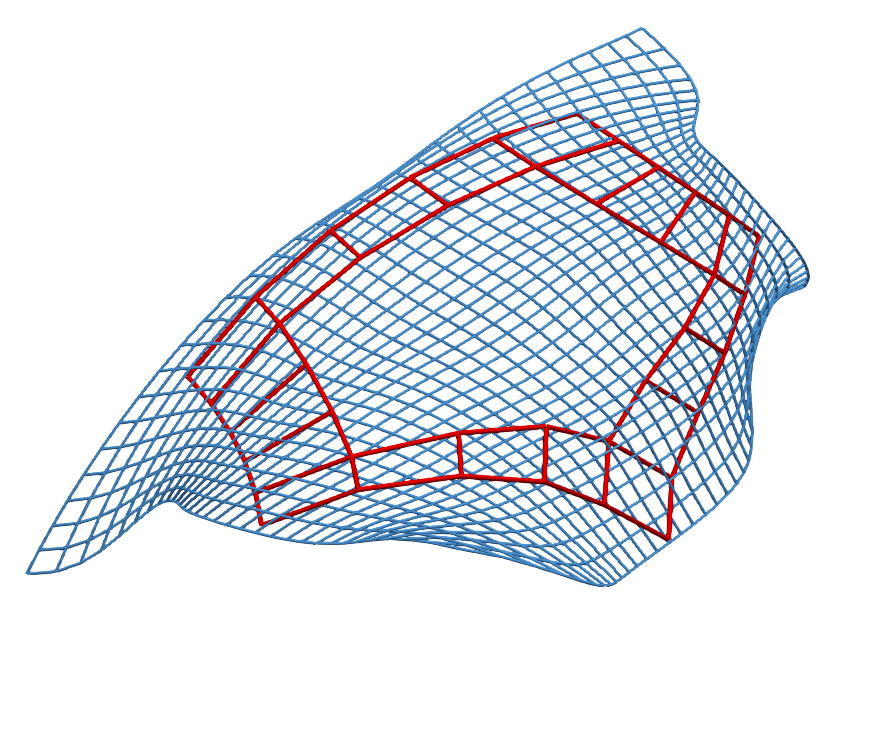
\includegraphics[width=\textwidth]{images/rotations/60.png}
      \caption{$\phi=60^\circ$}
    \end{subfigure}
    \hfill
    \begin{subfigure}{.26\textwidth}
      \centering
      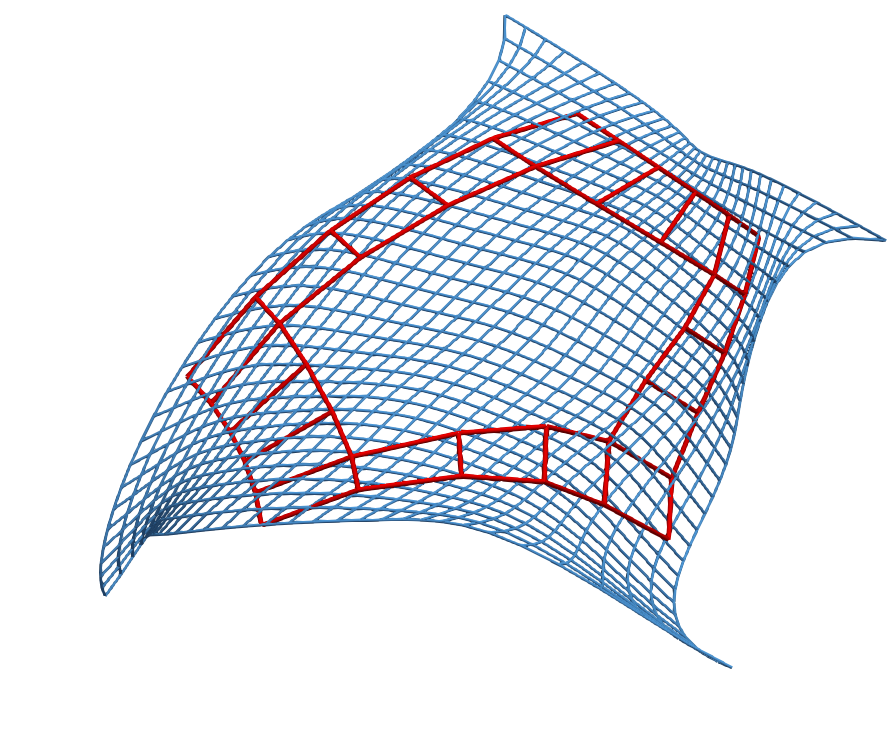
\includegraphics[width=\textwidth]{images/rotations/75-optimal.png}
      \caption{$\phi\approx 75^\circ$ (optimal)}
    \end{subfigure}
    \hfill
    \begin{subfigure}{.26\textwidth}
      \centering
      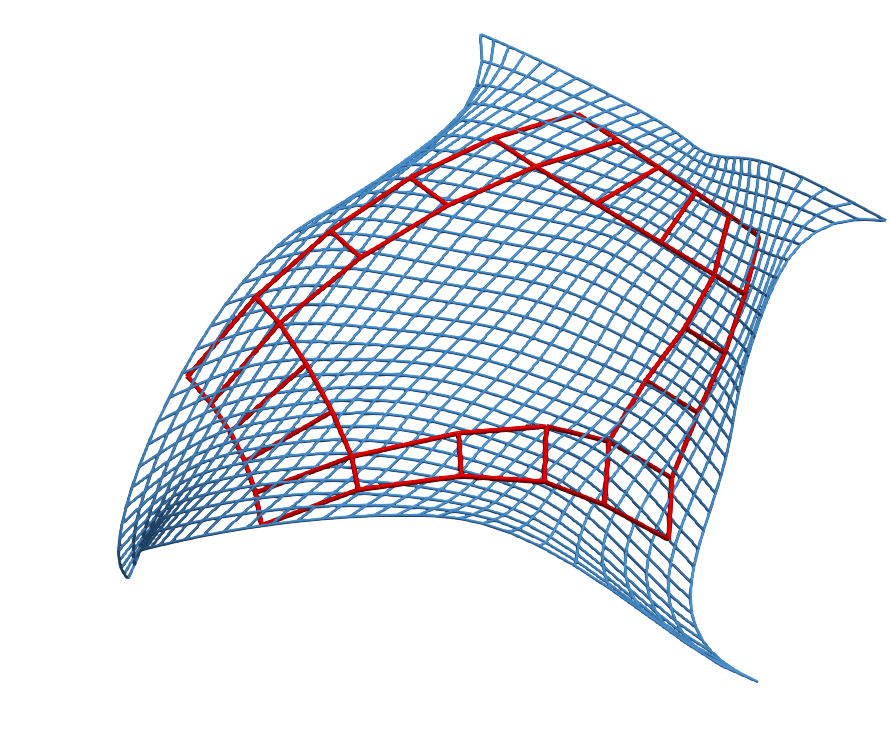
\includegraphics[width=\textwidth]{images/rotations/80.png}
      \caption{$\phi=80^\circ$}
    \end{subfigure}
    \hfill
  }

  \caption{The effect of rotating a 5-sided domain.}
  \label{fig:rotations}
\end{figure}
Rotating the domain, instead of scaling it, may also have a beneficial effect
on the control grid. However, in our experience, rotation of the domain in itself
is not sufficient to deal with 7- or 8-sided surfaces.
Figure~\ref{fig:rotations} shows several rotations of a 5-sided domain.
We can define the optimal rotation as one that minimizes the functional
\begin{equation}
  E = \sum_{i=0}^\delta\sum_{j=1}^{\delta-1}\left\|\frac{Q_{i,j-1}+Q_{i,j+1}}{2}-Q_{i,j}\right\|^2 +
  \sum_{i=1}^{\delta-1}\sum_{j=0}^\delta\left\|\frac{Q_{i-1,j}+Q_{i+1,j}}{2}-Q_{i,j}\right\|^2,
\end{equation}
where $Q_{i,j}$ are the control points of the bi-degree $\delta$ tensor product surface,
essentially selecting the smoothest control structure.

Table~\ref{tab:degrees} summarizes the degrees of all four representations.
It can be seen that these patches
have relatively high degrees, in particular when the number of sides and the degree of the
boundaries are raised. While Warren's patch outperforms the others in this respect,
the use of base points limits its usability in CAD systems.
Kato's surface always has singularities, and its degree is fairly high, but it is the only
construction where $G^2$ continuity can be easily achieved. We found that while the
Charrot--Gregory patch has a slightly higher degree than the S-patch, it has much lower
computational cost in its multi-sided form, and have no control net quality problems for
the most frequent 5- and 6-sided configurations.
\begin{table}
  \centering
  \begin{tabular}{c|c|c|c|c}
    $n$ & S-patch~\cite{Loop:1989} & Warren~\cite{Warren:1992} & Kato~\cite{Kato:1991} & Charrot--Gregory~\cite{Charrot:1984} \\ \hline
    3 & \multicolumn{2}{c|}{$d[+3]$ (both B\'ezier triangles)} & \cellcolor{light-gray}$3d+5$ & $d+3$ \\ \hline
    5 & \cellcolor{light-light-gray}$3d[+9]$ & $\approx 3d$ & \cellcolor{light-gray}$5d+9$ & $5d+6$ \\ \hline
    6 & \cellcolor{light-light-gray}$4d[+12]$ & $3d$ & \cellcolor{light-gray}$6d+11$ & $6d+8$ \\ \hline
    7+ & \cellcolor{light-gray}$(n-2)(d[+3])$ & $\qquad$N/A$\qquad$ & \cellcolor{light-gray}$nd+2n-1$ & \cellcolor{light-gray}$nd+2n-4$ \\ \hline
  \end{tabular}
  \caption{Rational polynomial degrees of the converted surfaces for different number of sides,
    assuming boundary curves of degree $d$. Gray cells indicate that the surface is susceptible to
    the singularity issue.
    For S-patches, the number in brackets is applied
    when the surface is generated by a degree-$d$ $G^1$ frame.}
  \label{tab:degrees}
\end{table}

\section{TEST CASES}
\label{sec:tests}
In this section we will show the rational B\'ezier conversion of more complex objects.
Since the tensor product surface is exactly the same as the multi-sided original,
there is little point in investigating the quality of the patches;
we are going to concentrate on the control net quality instead.
The domain-scaling method outlined above always generates nice control structures,
so a comparison using the default domain is more informative.
(We will show only S-patches and Charrot--Gregory patches,
because the other two surfaces always have singularities.)

All images in this section were created by a commercially available CAD system,
Rhinoceros 3D~\cite{Rhino3D}; the colors show mean curvature distribution,
patch boundaries and isocurves are drawn with black lines.

\begin{figure}[!ht]
  {
    \hfill
    \begin{subfigure}{.3\textwidth}
      \centering
      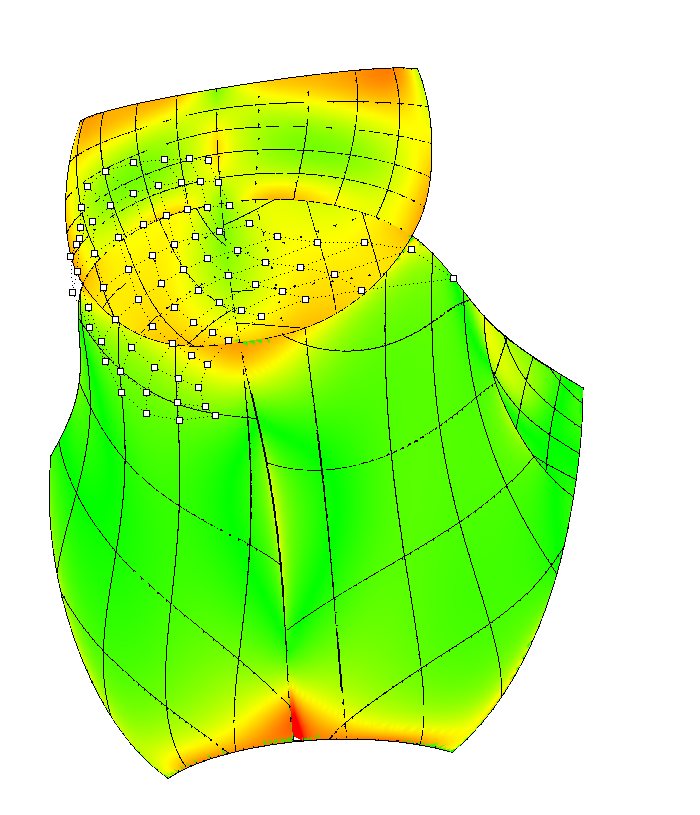
\includegraphics[width=.9\textwidth]{images/cagd86/spatch3.png}
      \caption{$n=3$, $\delta=8$}
      \label{fig:cagd86-3-sp}
    \end{subfigure}
    \hfill
    \begin{subfigure}{.3\textwidth}
      \centering
      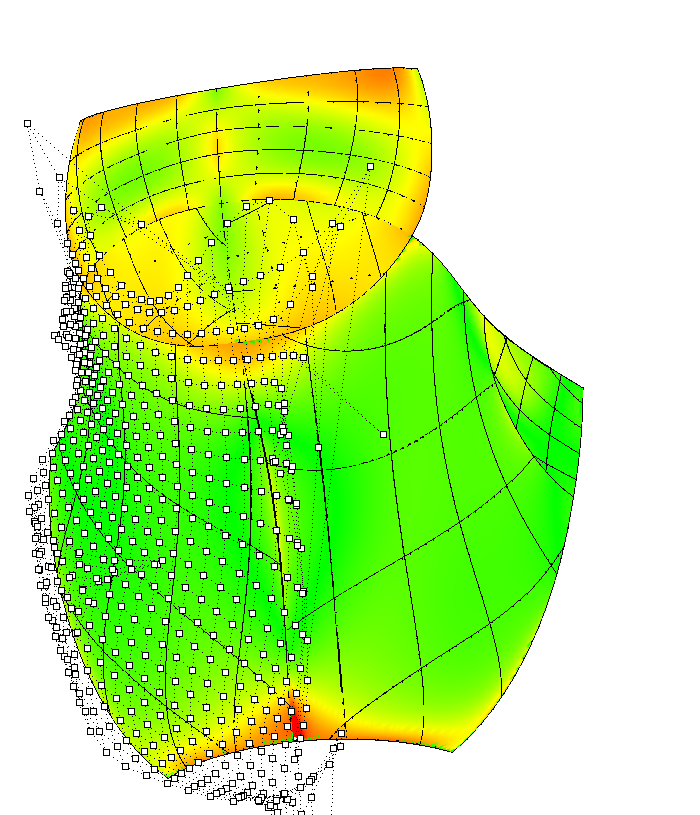
\includegraphics[width=.9\textwidth]{images/cagd86/spatch2.png}
      \caption{$n=5$, $\delta=24$}
      \label{fig:cagd86-5-sp}
    \end{subfigure}
    \hfill
    \begin{subfigure}{.3\textwidth}
      \centering
      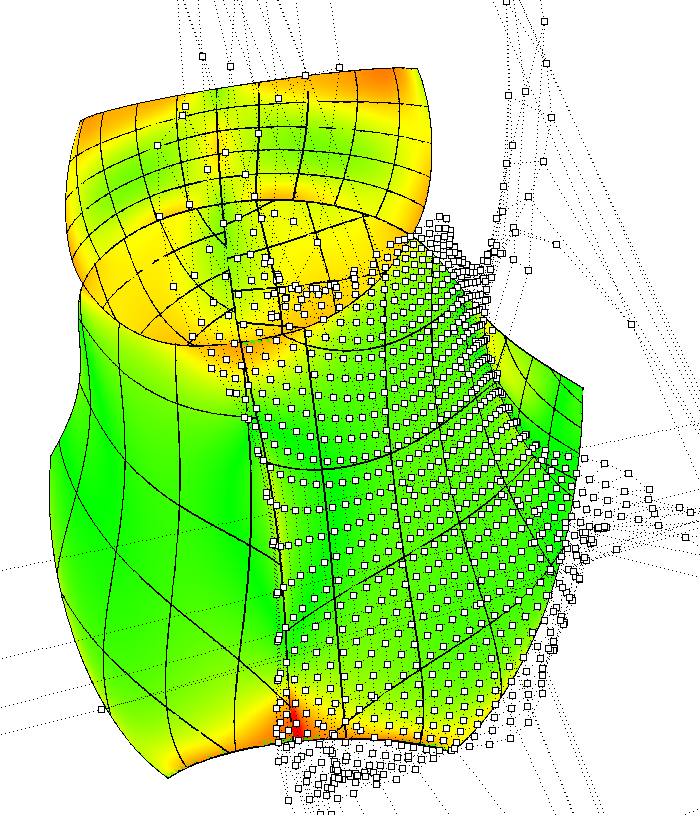
\includegraphics[width=.9\textwidth]{images/cagd86/spatch1.png}
      \caption{$n=6$, $\delta=32$}
      \label{fig:cagd86-6-sp}
    \end{subfigure}
    \hfill
  }

  {
    \hfill
    \begin{subfigure}{.3\textwidth}
      \centering
      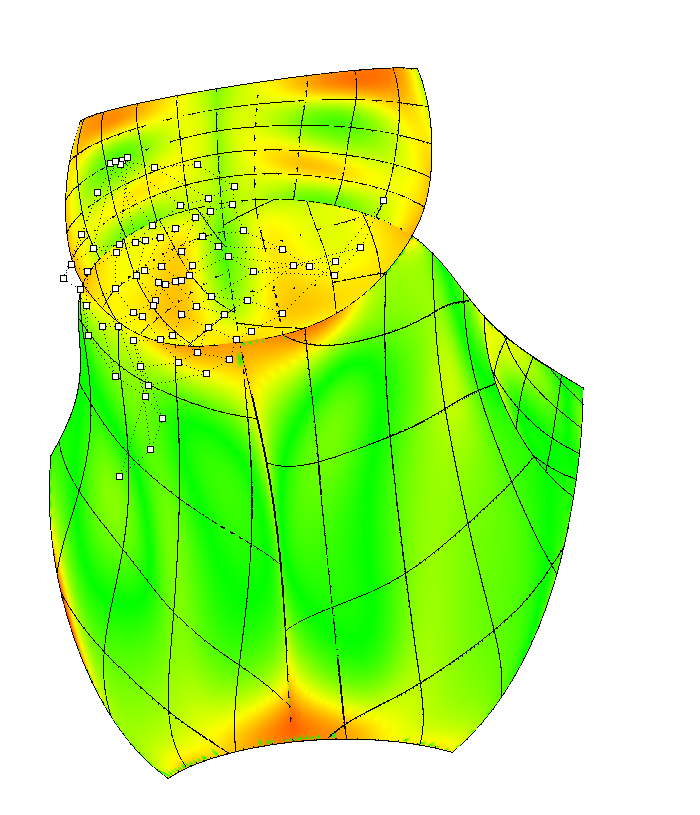
\includegraphics[width=.9\textwidth]{images/cagd86/cg3.png}
      \caption{$n=3$, $\delta=8$}
      \label{fig:cagd86-3-cg}
    \end{subfigure}
    \hfill
    \begin{subfigure}{.3\textwidth}
      \centering
      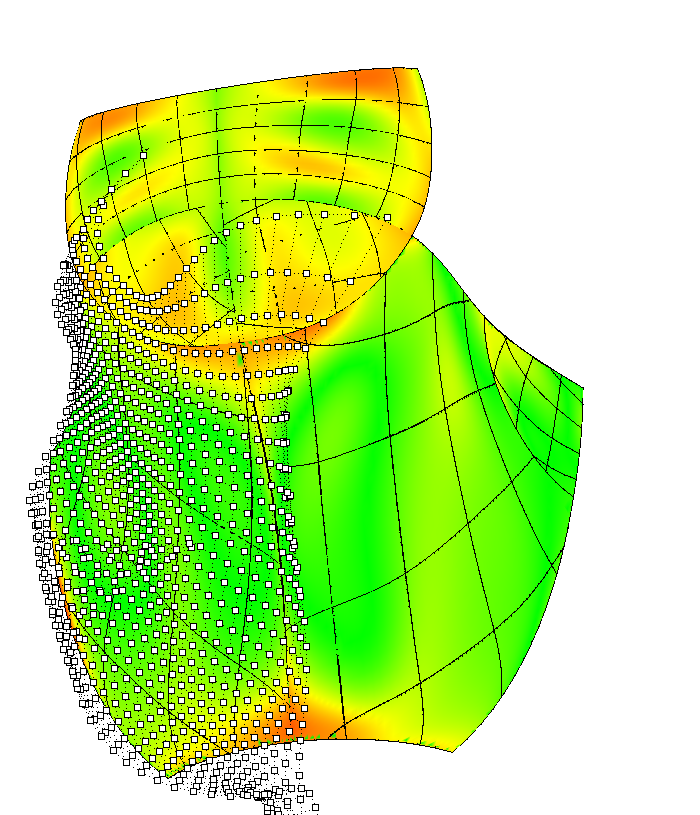
\includegraphics[width=.9\textwidth]{images/cagd86/cg2.png}
      \caption{$n=5$, $\delta=31$}
      \label{fig:cagd86-5-cg}
    \end{subfigure}
    \hfill
    \begin{subfigure}{.3\textwidth}
      \centering
      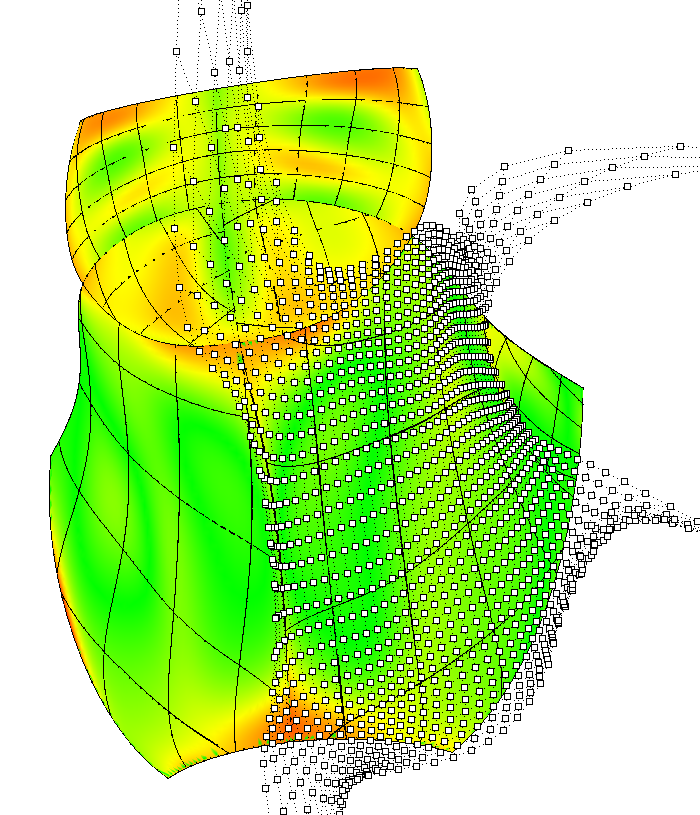
\includegraphics[width=.9\textwidth]{images/cagd86/cg1.png}
      \caption{$n=6$, $\delta=38$}
      \label{fig:cagd86-6-cg}
    \end{subfigure}
    \hfill
  }
  \caption{Control networks of S-patches (top) and Charrot--Gregory surfaces (bottom).}
  \label{fig:cagd86}
\end{figure}
The model in Figure~\ref{fig:cagd86}, defined by quintic $G^1$ frames,
has three 3-sided, two 4-sided, one 5-sided and one 6-sided surface.
The triangular S-patch shown in Fig.~\ref{fig:cagd86-3-sp} has a more regular
control net than its counterpart in Fig.~\ref{fig:cagd86-3-cg},
but the 5-sided patch in Fig.~\ref{fig:cagd86-5-sp}
shows some outliers compared to Fig.~\ref{fig:cagd86-5-cg},
and the 6-sided S-patch in Fig.~\ref{fig:cagd86-6-sp} has some
control points close to infinity, causing numerical evaluation errors
in the bottom-left corner, while the control net
in Fig.~\ref{fig:cagd86-6-cg}, deviating to some extent, is still managable.

\begin{figure}[!ht]
  \begin{subfigure}{.33\textwidth}
    \centering
    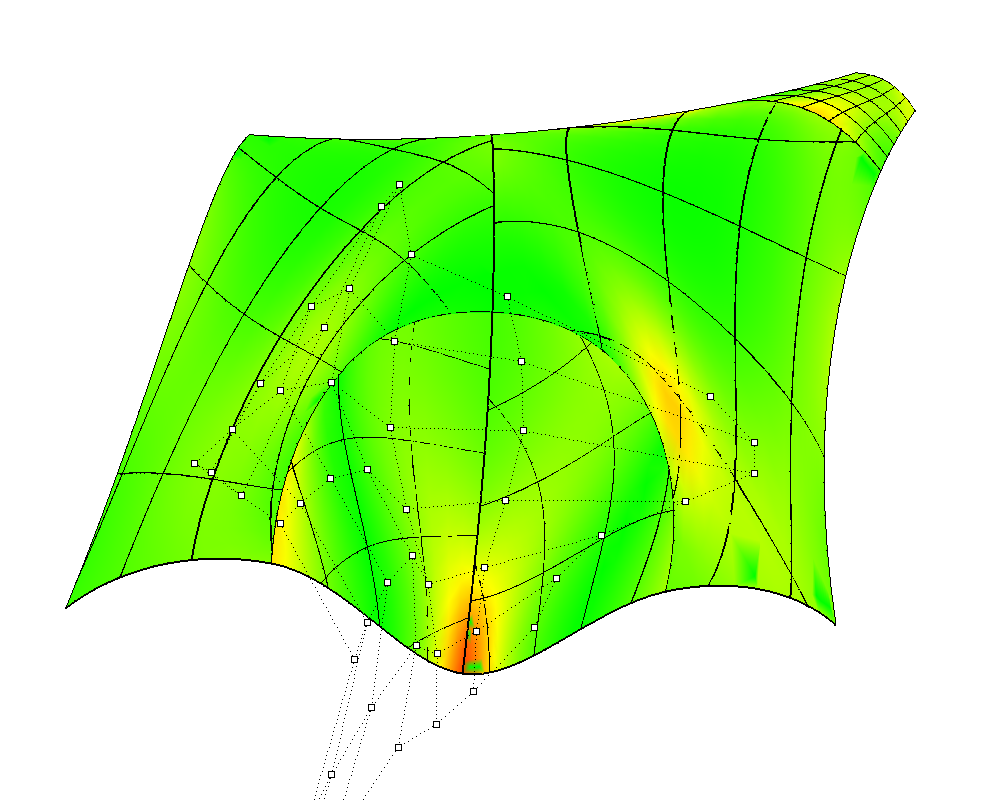
\includegraphics[width=\textwidth]{images/pocket/spatch3.png}
    \caption{$n=3$, $\delta=6$}
    \label{fig:pocket-3-sp}
  \end{subfigure}
  \begin{subfigure}{.33\textwidth}
    \centering
    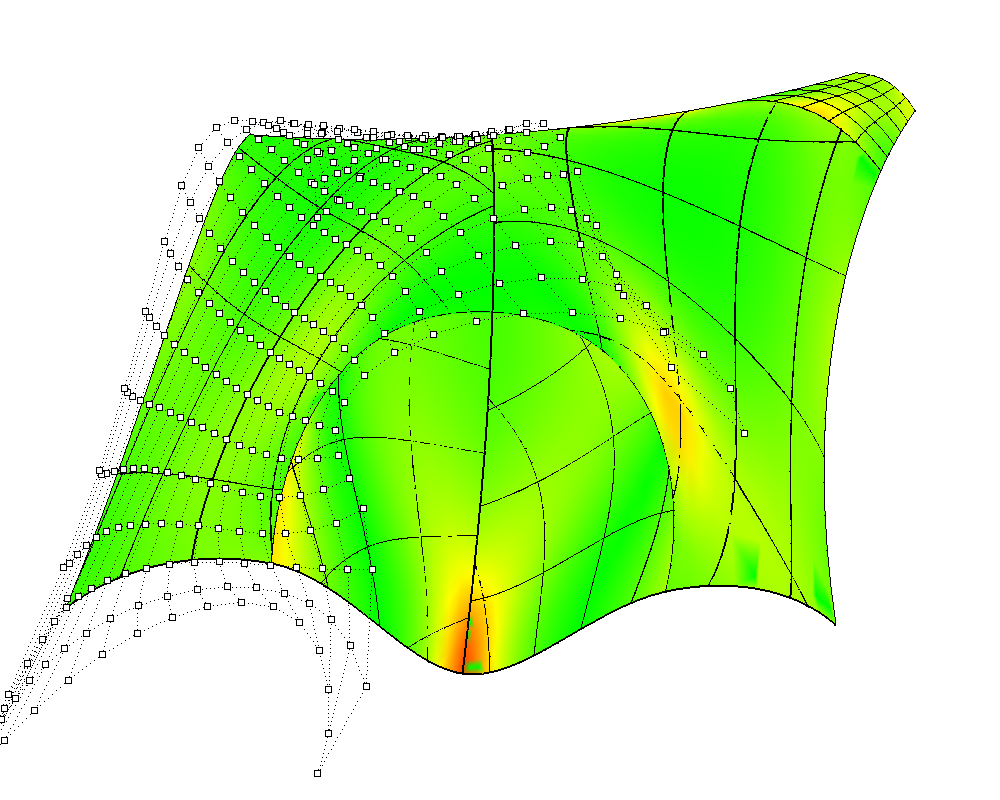
\includegraphics[width=\textwidth]{images/pocket/spatch2.png}
    \caption{$n=5$, $\delta=18$}
    \label{fig:pocket-5-sp}
  \end{subfigure}
  \begin{subfigure}{.33\textwidth}
    \centering
    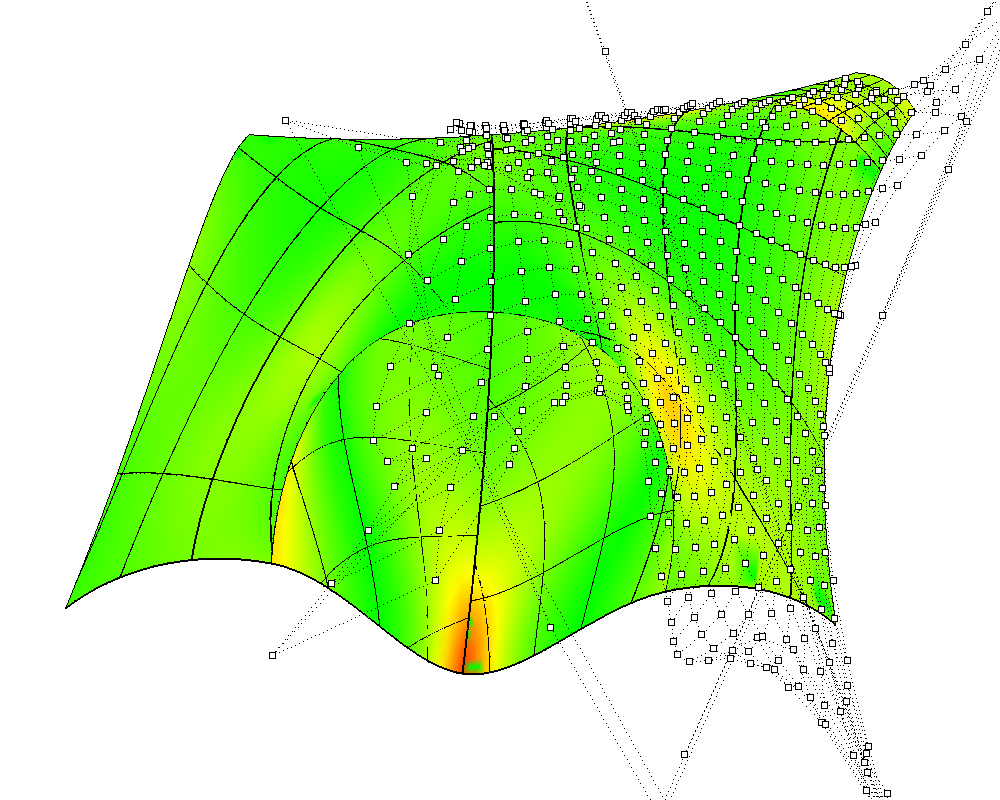
\includegraphics[width=\textwidth]{images/pocket/spatch1.png}
    \caption{$n=6$, $\delta=24$}
    \label{fig:pocket-6-sp}
  \end{subfigure}

  \begin{subfigure}{.33\textwidth}
    \centering
    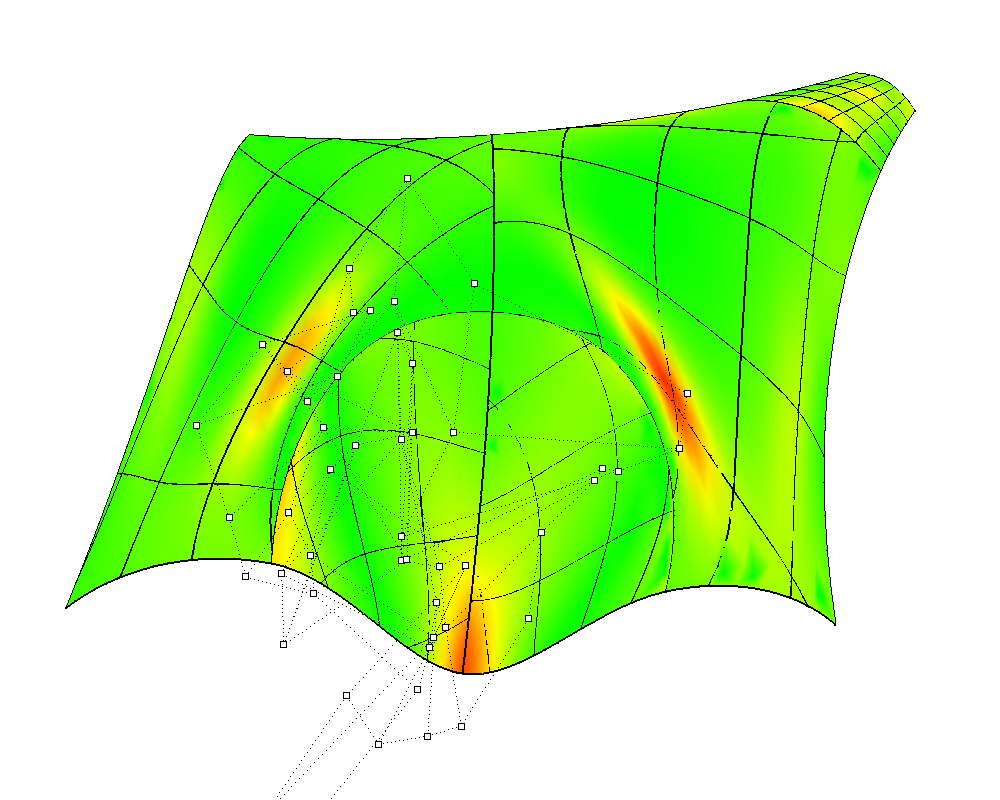
\includegraphics[width=\textwidth]{images/pocket/cg3.png}
    \caption{$n=3$, $d=6$}
    \label{fig:pocket-3-cg}
  \end{subfigure}
  \begin{subfigure}{.33\textwidth}
    \centering
    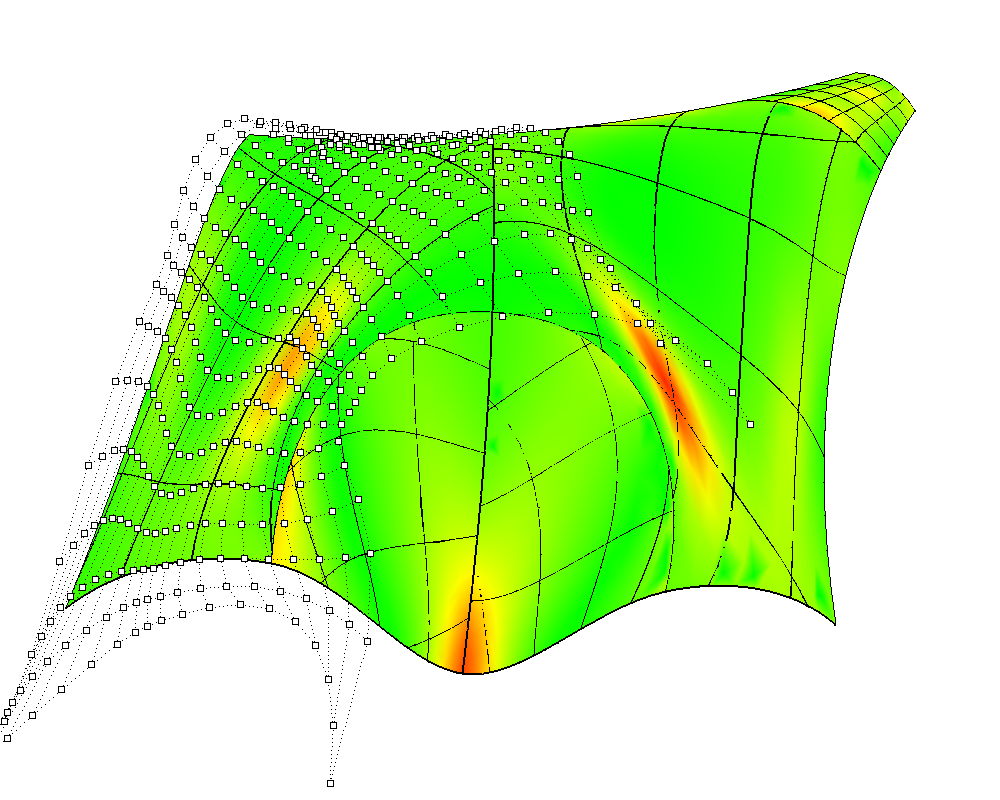
\includegraphics[width=\textwidth]{images/pocket/cg2.png}
    \caption{$n=5$, $\delta=21$}
    \label{fig:pocket-5-cg}
  \end{subfigure}
  \begin{subfigure}{.33\textwidth}
    \centering
    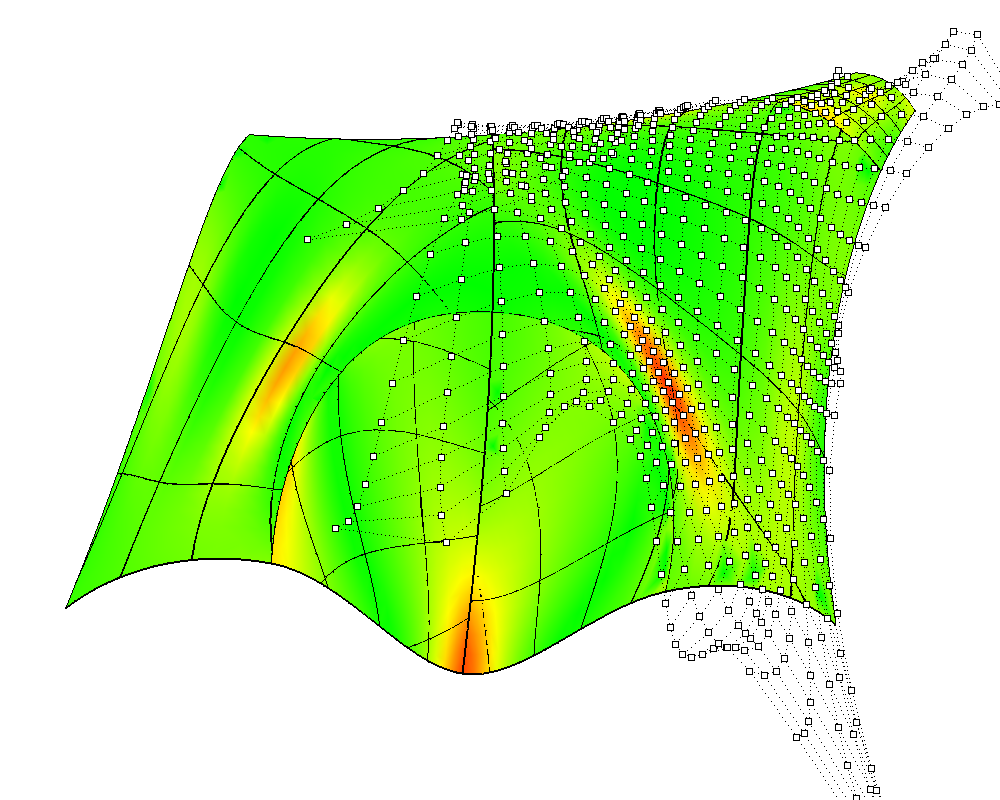
\includegraphics[width=\textwidth]{images/pocket/cg1.png}
    \caption{$n=6$, $\delta=26$}
    \label{fig:pocket-6-cg}
  \end{subfigure}
  \caption{``Pocket'' model (top: S-patches, bottom: Charrot--Gregory patches).}
  \label{fig:pocket}
\end{figure}

We find similar results in the ``Pocket'' model (Figure~\ref{fig:pocket}),
where the surfaces were defined by cubic $G^1$ frames, and are of a lower degree.
In this case the irregularities in the control net of the 6-sided S-patch
did not lead to any evaluation problems.

Finally, in Figure~\ref{fig:dolphin}, a dolphin model
is shown, defined by quintic $G^1$ frames. The two 6-sided S-patches are
not evaluated correctly here due to the erratic control points.
One of the Charrot--Gregory patches also stretches far near the corners,
but is still within the limits of exact evaluation.
\begin{figure}[!ht]
  {
    \hfill
    \begin{subfigure}{.45\textwidth}
      \centering
      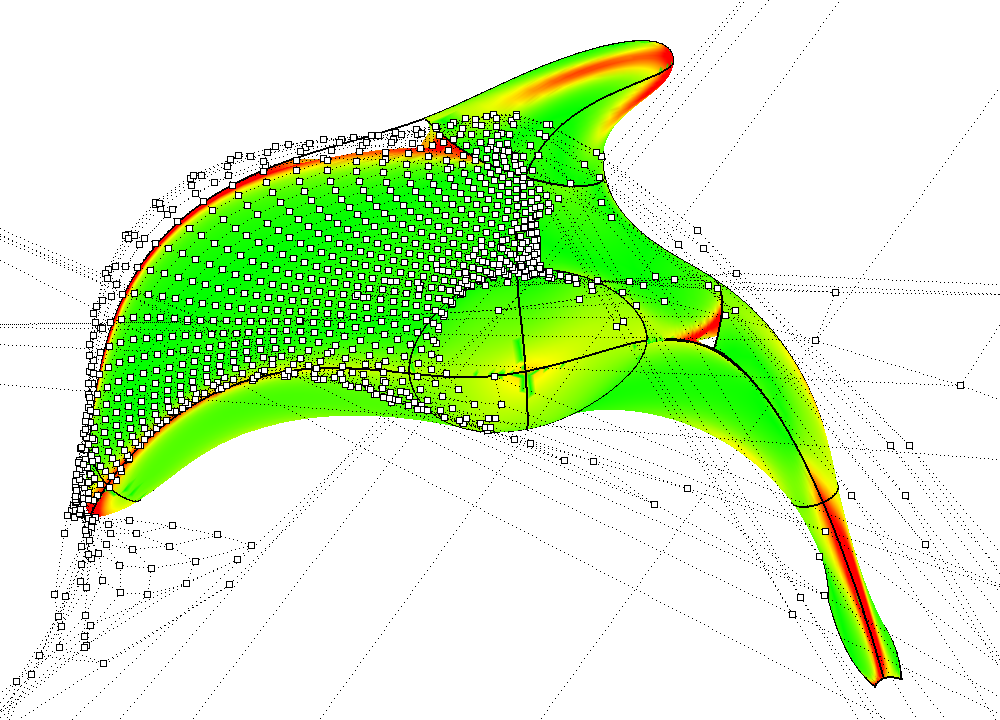
\includegraphics[width=\textwidth]{images/dolphin/spatch1.png}
      \caption{$n=6$, $\delta=32$}
      \label{fig:dolphin-3-sp}
    \end{subfigure}
    \hfill
    \begin{subfigure}{.45\textwidth}
      \centering
      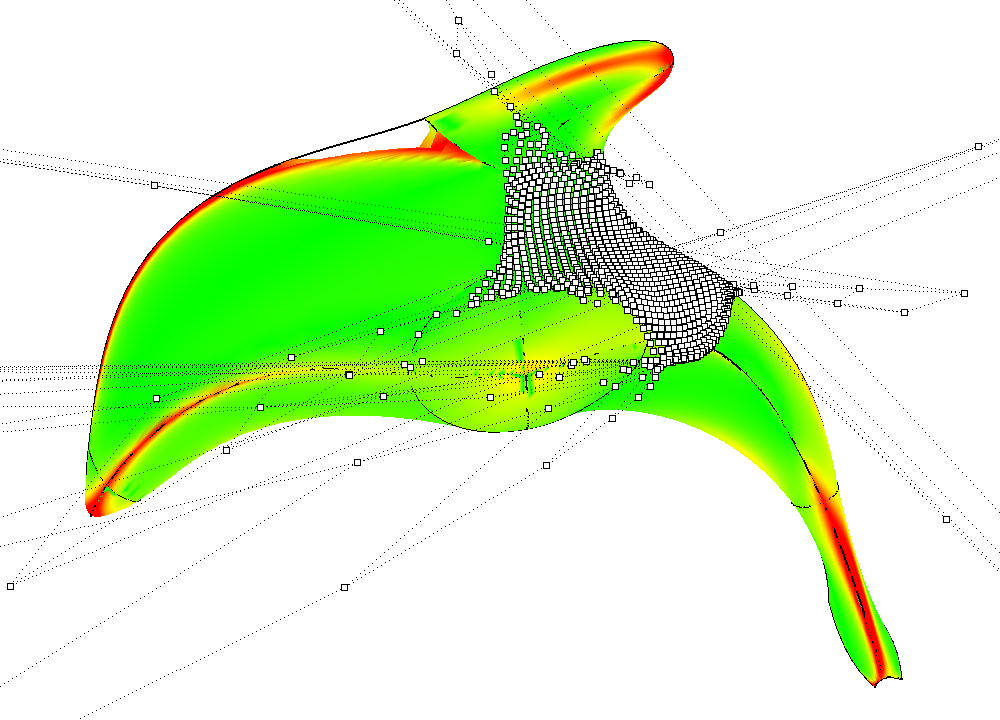
\includegraphics[width=\textwidth]{images/dolphin/spatch2.png}
      \caption{$n=6$, $\delta=32$}
      \label{fig:dolphin-5-sp}
    \end{subfigure}
    \hfill
  }

  {
    \hfill
    \begin{subfigure}{.45\textwidth}
      \centering
      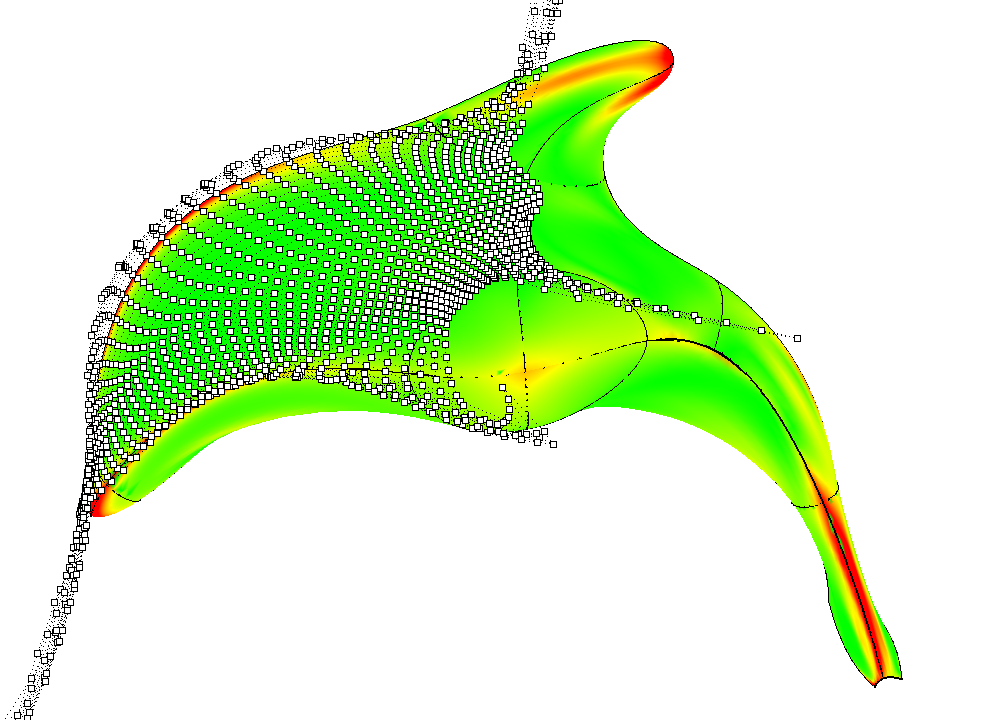
\includegraphics[width=\textwidth]{images/dolphin/cg1.png}
      \caption{$n=6$, $\delta=38$}
      \label{fig:dolphin-3-cg}
    \end{subfigure}
    \hfill
    \begin{subfigure}{.45\textwidth}
      \centering
      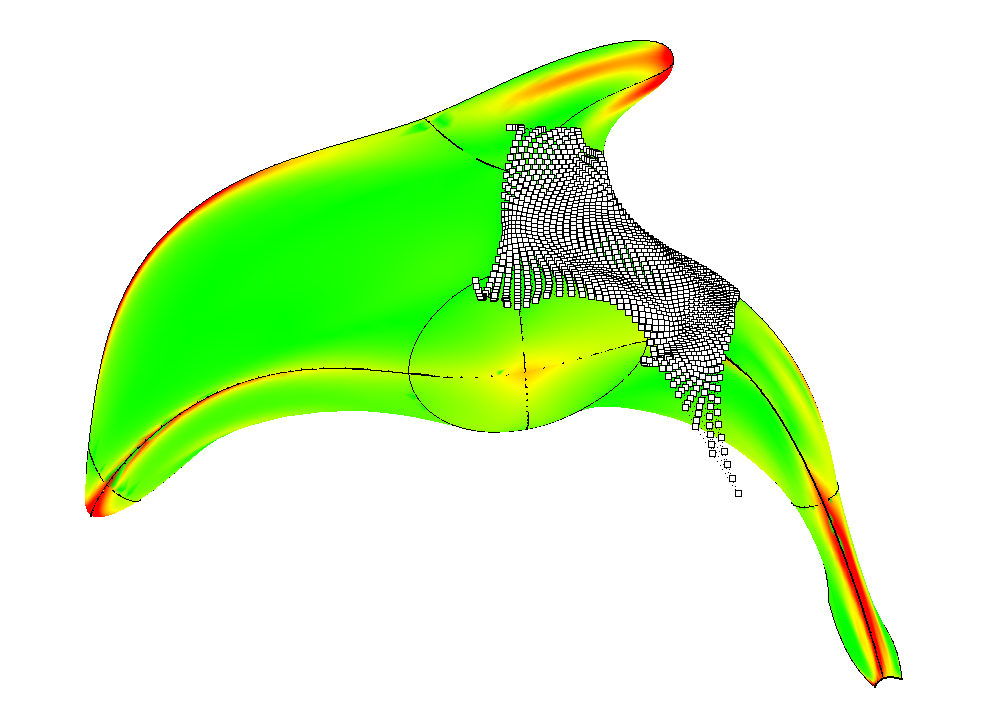
\includegraphics[width=\textwidth]{images/dolphin/cg2.png}
      \caption{$n=6$, $\delta=38$}
      \label{fig:dolphin-5-cg}
    \end{subfigure}
    \hfill
  }
  \caption{Dolphin model (top: S-patches, bottom: Charrot--Gregory patches).}
  \label{fig:dolphin}
\end{figure}

\section{CONCLUSIONS}
We have described and analyzed four genuine multi-sided surface representations
that can be converted into standard, tensor product (rational B\'ezier) form.
The conversion generally leads to high-degree patches, and the
control points of the resulting surfaces may oscillate, due to singularities,
to an extent that prevents practical usability in industrial CAD/CAM systems.

We have investigated the occurrence of singularities for these schemes,
and introduced a technique to avoid nonsense control structures.
Using the proposed exact conversion procedures one can build watertight
and smoothly connected models with trimmed surface patches.

All four schemes presented in this paper have their deficiencies; however, our
practical experience would assign some advantage to Charrot--Gregory
patches. We are going to continue searching for other patch representations
that possess both multi-sided shape control and low-degree tensor product form.

\section*{ACKNOWLEDGEMENTS}
This project has been supported by the Hungarian Scientific Research Fund (OTKA, No.~124727)%
, and the National Research, Development and Innovation Fund (TUDFO/51757/2019-ITM,
Thematic Excellence Program)%
.

\section*{ORCID}
\orcid{P\'eter Salvi}{0000-0003-2456-2051}
\orcid{Tam\'as V\'arady}{0000-0001-9547-6498}

\appendix
\section{CONVERSION EQUATIONS}
\label{app:conversion-eqs}
The following appendices show the patch equations
with the numerator and denominator separated,
so the tensor product conversion can be done
according to Eqs.~(\ref{eq:power}--\ref{eq:bernstein}).

\subsection*{Kato's Patch}
The blending functions have the same denominators, but the side parameters do not.
Introducing the notation $\mathcal{L}_i=L_{i-1}+L_{i+1}$, and omitting the
parameters for brevity, the patch equation becomes
\begin{equation}
  S_\mathrm{Kato}=
  \frac{1}{\sum_{i=1}^nH_i^{e+1}}\cdot
  \sum_{i=1}^n\sum_{j=0}^d\sum_{k=0}^{e}
  P_{j,k}^i\cdot
  {d\choose j}\frac{L_{i-1}^j}{\mathcal{L}_i^j}\frac{L_{i+1}^{d-j}}{\mathcal{L}_i^{d-j}}\cdot
  {e\choose k}L_i^k(1-L_i)^{e-k}
  \cdot H_i^{e+1}.
\end{equation}
Dividing and multiplying the equation with $\prod_{i=1}^n\mathcal{L}_i^d$, we arrive at the form
\begin{align}
  \begin{split}
    S_\mathrm{Kato}=
    &\frac{1}{\sum_{i=1}^nH_i^{e+1}}\cdot
    \frac{1}{\prod_{i=1}^n\mathcal{L}_i^d}\cdot
    \sum_{i=1}^n\sum_{j=0}^d\sum_{k=0}^{e}
    P_{j,k}^i\cdot\\
    &\left[{d\choose j}\cdot L_{i-1}^jL_{i+1}^{d-j}\prod_{\substack{r=1\\r\neq i}}^n\mathcal{L}_r^d\right]
    \cdot {e\choose k}L_i^k(1-L_i)^{e-k}
    \cdot H_i^{e+1}.
  \end{split}
\end{align}

\subsection*{Charrot--Gregory Patch}
Similarly to Kato's patch, straightforward calculation leads to the form
\begin{equation}
  S_\mathrm{CG}= \frac{1}{\sum_{i=1}^nH_{i-1,i}^2}\cdot \frac{1}{\prod_{i=1}^n\mathcal{L}_i^d}\cdot
  \sum_{i=1}^n\left[\hat{R}_{i-1}+\hat{R}_i-\hat{Q}_{i-1,i}\right]
  \cdot H_{i-1,i}^2
  \cdot\prod_{\substack{r=1\\r\neq i-1,i}}^n\mathcal{L}_r^d,
\end{equation}
where
\begin{align}
  \hat{R}_{i-1}=&\sum_{j=0}^d
  \left[P_{j0}^{i-1}\mathcal{L}_i+L_{i-1}d(P_{j1}^{i-1}-P_{j0}^{i-1})\right]\cdot
  {d\choose j}L_{i-2}^jL_i^{d-j}\mathcal{L}_i^{d-1},\\
  \hat{R}_i=&\sum_{j=0}^d
  \left[P_{j0}^i\mathcal{L}_{i-1}+L_id(P_{j1}^i-P_{j0}^i)\right]\cdot
  {d\choose j}L_{i-1}^jL_{i+1}^{d-j}\mathcal{L}_{i-1}^{d-1},\\
  \begin{split}
    \hat{Q}_{i-1,i}=&
    \big[P_{00}^i\mathcal{L}_{i-1}\mathcal{L}_i+L_{i-1}d(P_{10}^i-P_{00}^i)\mathcal{L}_{i-1}+
      L_id(P_{01}^i-P_{00}^i)\mathcal{L}_i+\\
      &\ \,L_{i-1}L_id^2(P_{11}^i-P_{10}^i-P_{01}^i+P_{00}^i)\big]\cdot
    \mathcal{L}_{i-1}^{d-1}\mathcal{L}_i^{d-1}.
  \end{split}
\end{align}

\section{TRIANGULAR CHARROT--GREGORY PATCH}
\label{app:triangular}
Substituting $h_{i-1}$ and $h_i$ for $s_i$ and $1-s_{i-1}$, respectively, the patch equation becomes
\begin{equation}
  S_\mathrm{CG_\triangle}= \frac{1}{\sum_{i=1}^3H_{i-1,i}^2}\cdot
  \sum_{i=1}^3\left[R_{i-1}(1-h_i,h_{i-1})+R_i(h_{i-1},h_i)-Q_{i-1,i}(1-h_i,h_{i-1})\right]
  \cdot H_{i-1,i}^2,
\end{equation}
which is directly convertable to tensor product form. While this is of a much lower degree
than the original parameterization, it cannot be used for $n>3$, because then
$h_i$ may take on values larger than $1$, and thus the ribbons would be evaluated outside
the $[0,1]$ interval, which can damage surface quality.

\referenceSection
\bibliographystyle{CADA}
\bibliography{cikkek}

\bigskip
\end{document}
